\documentclass[11pt]{article}
\usepackage{svg}
\usepackage{graphbox}
\usepackage{multicol}
\usepackage{amsmath}
%\usepackage{siunitx}
\usepackage{ulem}
\usepackage{amssymb}
\usepackage{mathtools}
\usepackage{appendix}
\usepackage{pgfplots}
\usepackage{subfig}
\usepackage{braket}
\usepackage{import}
\usepackage{cancel}
\usepackage{xcolor,colortbl}
\usepackage[colorlinks=true, allcolors=blue]{hyperref}
\usepackage{mathtools}
\usepackage[export]{adjustbox}
\usepackage{enumitem}
\usepackage{graphicx}
\usepackage[font=small,labelfont=bf]{caption}
\usepackage{subfig}
%\usepackage{caption}
%\usepackage{subcaption}
%\usepackage{subfigure}
%\usepackage{fancyhdr}
%\pagestyle{fancy}
%\fancyhf{}
%\cfoot{}

\newcommand{\sig}{\overline{\sigma}_i}
\newcommand{\eq}{=&\ }
\newcommand{\ints}{\int\displaylimits_\sigma}
\newcommand{\intm}{\int\displaylimits_\mu}
\newcommand{\on}{\mathcal{O}(N)}
\newcommand{\onlogn}{\mathcal{O}(N\log(N))}
\setlist{  
	listparindent=\parindent,
	parsep=0pt,
}

\author{Sean Baccas}


\oddsidemargin=-.3in
\evensidemargin=-.5in
\textwidth=7in
\topmargin=-1in
\textheight=9.7in

\parindent=.3in
\pagestyle{plain}

\definecolor{Gray}{gray}{0.9}
\definecolor{Yellow}{rgb}{255,255,0}
%\newcolumntype{y}{>{\columncolor{Yellow}}c}

\allowdisplaybreaks

\newenvironment{problems}
{
	\begin{enumerate}
		\renewcommand{\labelenumi}{ {\bf \arabic{enumi}}.}
		\setlength{\itemsep}{0.5em}
	}
	{
	\end{enumerate}
}

\newcommand{\nn}{\nonumber}

%BASE WORD COUNT IS 12


\begin{document}
	% Last modification: 2015-08-17 (Marc Deisenroth)
\begin{titlepage}

\newcommand{\HRule}{\rule{\linewidth}{0.5mm}} % Defines a new command for the horizontal lines, change thickness here


%----------------------------------------------------------------------------------------
%	LOGO SECTION
%----------------------------------------------------------------------------------------

\includegraphics[width = 4cm]{./figures/imperial}\\[0.5cm] 

\center % Center remainder of the page

%----------------------------------------------------------------------------------------
%	HEADING SECTIONS
%----------------------------------------------------------------------------------------

\textsc{\Large Imperial College London}\\[0.5cm] 
\textsc{\large Department of Physics}\\[0.5cm] 

%----------------------------------------------------------------------------------------
%	TITLE SECTION
%----------------------------------------------------------------------------------------

\HRule \\[0.4cm]
{ \huge \bfseries Bayesian Cluster Analysis for Super Resolved Microscopy}\\ % Title of your document
\HRule \\[1.5cm]
 
%----------------------------------------------------------------------------------------
%	AUTHOR SECTION
%----------------------------------------------------------------------------------------

\begin{minipage}{0.4\textwidth}
\begin{flushleft} \large
\emph{Author:}\\
Sean Baccas % Your name
\end{flushleft}
\end{minipage}
~
\begin{minipage}{0.4\textwidth}
\begin{flushright} \large
\emph{Supervisor:} \\
Prof. Paul French and Dr Andrew Rose% Supervisor's Name
\end{flushright}
\end{minipage}\\[4cm]


%----------------------------------------------------------------------------------------
%	FOOTER & DATE SECTION
%----------------------------------------------------------------------------------------
\vfill % Fill the rest of the page with whitespace
A thesis submitted in partial fulfilment of the
requirements for the degree of Master of Physics with Quantum Dynamics and the
Diploma of Imperial College London.\\[0.5cm]

\makeatletter
\today 
\makeatother


\end{titlepage}

	\textbf{Acknowledgments}

I'd like to thank Dr Andrew Rose for his guidance throughout this project, without which this project would not have been possible. Secondly, I'd to thank MiQi Lim for her help in deciphering all the biological aspects of this project. Finally, I'd like to thank Tim Heightman, for his keen eyes proofreading this project, and for getting me through this master's degree.\\

\textbf{Declaration}
I declare that the work presented in this thesis was entirely written by me, and will not be used for other academic purposes. Any materials protocols, algorithms and previously written code have been correctly cited. The bulk of the implementation was undertaken by Dr Andrew Rose before the beginning of this project, namely the identification of useful algorithmic speed-ups, the conversion of raw data into equivalent, lightweight forms, and the introduction of multi-threading. The contribution of this report is the verification of the function of the software, both through debugging and analysing SMLM data using this procedure. 
The contents of this report are entirely my own.

	
% 	\begin{center}
% 		{\Large \bf Bayesian Clustering for Single Molecule Localisation Microscopy} \smallskip
		
% 		{\Large \em %Nueva Multivariable Calculus, Fall 2021
			
			
			
% 			%DAY MONTH, 2021
			
% 		}
% 		Sean Baccas\\
% 		Supervised by Professor Paul French and Dr Andrew Rose
% 	\end{center}
	\begin{abstract}
		
		In recent years, the advent of single-molecule localisation microscopy (SMLM) \cite{Lelek2021} has enabled imaging of biological systems beyond the limit of the camera resolutions. In this review, we aim to describe SMLM, and motivate the need for identifying clusters within the data. 
		%stuff to answer:\\
		%\begin{enumerate}
		%	\item how is fluorescence achieved?
		%	\item what is clustering?
		%	\item note that it won the nobel prize
		%	\item analysing the data is tricky because they all fluoresce at the same time etc
		%	\item we need to talk about STORM and THUNDERSTORM
		%	\item we have lots of things together and take 5000 frames to make sure we see each molecule flash once
		%\end{enumerate}
		
	\end{abstract}	
	
	\tableofcontents
	

% we don't want to have to use electron microscopes!!\\
\newpage
\section{Introduction}
Single-Molecule Localisation Microscopy (SMLM) has, in recent years, greatly enhanced the capabilities of biologists to observe the dynamics and characteristics of biological processes within cells. Techniques such as STORM \cite{rust2006sub} enable users to fluorescent molecules (fluorophores) with resolutions in the tens of nanometres, and techniques such as ThunderSTORM \cite{thunderstorm} allow for the construction of large datasets that describe in detail the full list of molecules in the Field of View (FOV). Such a dense, granular description of the data has enabled advances in the study of biological systems. For a full review of this topic, see reference \cite{Lelek2021}.\\

With such dense datasets comes the need to analyse the data quantitatively and qualitatively, but the number of points involved can make this prohibitive to do from a computational standpoint. This report concerns itself with searching for descriptors for how various molecules are \textit{clustered} together in the images produced of biological samples. What constitutes a cluster in this context is not always easy to define, but broadly speaking, a cluster is an area of an image that contains a group of molecules that appear to be closer to each other than to any other of their other nearest neighbours. The characteristics of the clusters of certain molecules, such as their width, density, and prevalence within a sample can lead to important insights into the underlying biology within an image. A full review of the analysis of SMLM clusters can be found in \cite{Khater2020}.\\

One method of note for identifying clusters can be found in reference \cite{Rubin-Delanchy2015}. This procedure uses a simple, geometric process for \textit{proposing} clusters, based on the work of \cite{getisAndFranklin}. They combine this with a Bayesian method for evaluating whether proposed clusters conform to some expected model characteristics, such as their shape, width and density when compared with the background. The most important characteristic of a cluster is that it is in some way distinguishable from complete spatial randomness (CSR), and this report shall outline the reasoning behind the method used in \cite{Rubin-Delanchy2015}, carried forward from \cite{getisAndFranklin}. \\

Until this point, implementations of this method of identifying clusters have not been suitable for use on large datasets. The authors of \cite{Rubin-Delanchy2015}, in a follow-up paper \cite{griffie2016bayesian}, note that the analysis of a region containing 1000 points (hereafter referred to as localisations) takes 30 minutes on a standard office desktop. Typical SMLM data can contain millions of localisations, with runtimes stretching to several hours. The main contribution is the implementation and verification of high-performance code to undertake this procedure. 





\newpage
\section{Fluorescence Microscopy and SMLM}
Fluorescence microscopy is a broad field of study that handles imaging of biological samples on a sub-micrometre scale. For a thorough review of the topic, please refer to \cite{combs2017current, pFrenchReview}. Whilst the function of modern microscopes is relatively similar to previous eras, what has changed is the ability to examine fluorescence coming directly from molecules of interest. This allows for the study of the spatial and temporal dynamics of the processes that occur within cells. One key development has been the use of different \textit{fluorophores}, fluorescent proteins which can be attached to molecules of interest. The wavelengths of light they emit can provide key indicators of the dynamics. In particular, proteins such as Alexa-647 and Cy5 can be efficiently attached to cellular molecules of interest, producing emissions when stimulated to do so by laser light of the correct wavelength.\\

Fluorescence microscopy is limited in its resolution. Due to diffraction that occurs as light reaches the focal plane, the smallest resolvable objects are around 200nm. Below this, fluorophores appear as a blurry point spread function (PSF), as shown in figure 1. The pattern observed is an Airy disk, with a full width half maximum of approximately $\lambda / 2\cdot NA$, where $0.2 < NA < 1.5$ is the numerical aperture of the microscope\cite{pFrenchReview}.  Airy functions are usually expressed in terms of modified Bessel functions, expressed in terms of infinite sums, and the $\Gamma$ function, the analytic continuation of the factorial function. We find that in most contexts, approximation with a Gaussian model, like the one described in ref. \cite{SCHOWENGERDT200775} is sufficient for most cases. \\



\begin{figure}[b!]
	\centering
	\subfloat[\centering Blurred image of a fluorescent molecule. ]{{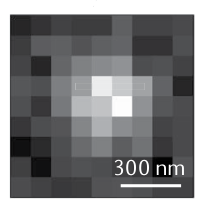
\includegraphics[width=0.4\textwidth]{figs/PSF.png} }}
	\qquad
	\subfloat[\centering Perturbing the location of a fluorophore leads to a predictable change in the detected pixel values. ]{\raisebox{10ex}{{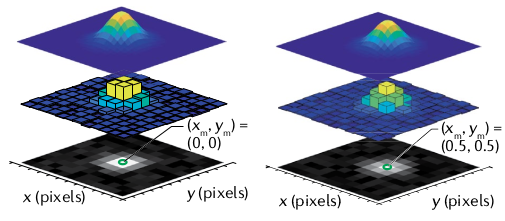
\includegraphics[width=0.4\textwidth]{figs/pixelShift.png} }}}
	\caption{A demonstration of SMLM, from \cite{Lelek2021}. On the left, we see a diffraction-limited image of a fluorophore. Due to the wavelength of the light emitted, and the optical equipment in use, diffraction means the object is to small to be resolvable at this scale, with the minimum resolving size being in the hundreds of nanometres. What we see instead is a blurred, bright spot in the centre of the image. In higher resolutions, one would observe an Airy pattern of concentric rings, decreasing in brightness. The figure on the right shows that a small perturbation of the location of a fluorophore leads to a predictable change in the measured pixel values \cite{Lelek2021}. This means that despite the site of the fluorescence being unobservable directly, we can accurately determine its coordinates to within a few tens of nanometres.}%
\label{pixelShift}
\end{figure}


Overcoming the diffraction limit in fluorescence microscopy can either be achieved through the costly and time-intensive use of electron microscopes, or through techniques known as Single Molecule Localisation Microscopy (SMLM) \cite{rust2006sub, Lelek2021} The idea behind SMLM is as follows: so long as fluorophores are sufficiently separated in space, or are not fluorescing simultaneously, then their spatial coordinates can be determined to a precision in the tens of nanometres - a much higher resolution than the approximately 200nm width of most relevant PSFs. One key technique in this domain is
Stochastic Optical Reconstruction Microscopy (STORM) \cite{rust2006sub}, which would go on to win the 2014 Nobel prize in Chemistry. As the authors mention, individual molecule positions can be determined to high accuracy with sufficiently many photons, but this does not directly translate into higher-resolution imaging techniques as multiple fluorophores nearby each other will be difficult to resolve \cite{rust2006sub}. The STORM method circumvents this by ensuring that fluorescent molecules are stochastically switched on and off, with the eventual image being aggregated from many different frames, with the aim being that only one fluorophore is blinking per frame in each diffraction-limited of the field of view. Each molecule is labelled with a photoswitchable dye, meaning that it can be stimulated into emitting a photon when illuminated with laser of a particular wavelength. Rust et al. use Cy5, a cynanine dye which they demonstrate can be encouraged to fluoresce, or sent back to a dark state, in a consistent pattern.  \cite{rust2006sub, cyanineDye}. Xu et al. \cite{stormAndThunderstorm} give a good review of the considerations that must be made when attempting to label photo-switchable fluorophores onto the molecular target of interest. The specific details of the process of undertaking SMLM imaging is beyond the scope of this report.\\ 
%\subsubsection{Some notes on the Lelek review}

\subsection{Photoswitching and Dyes}
% \textbf{todo}:
% \begin{itemize}
% 	\item not sure if \textbf{stimulated} is the right word
% 	\item review the paper in the comment under the fig
% 	\item this part should be about dye selection and how to label - might not be that detailed.
% \end{itemize}
\begin{figure}[h!] 
	\centering
	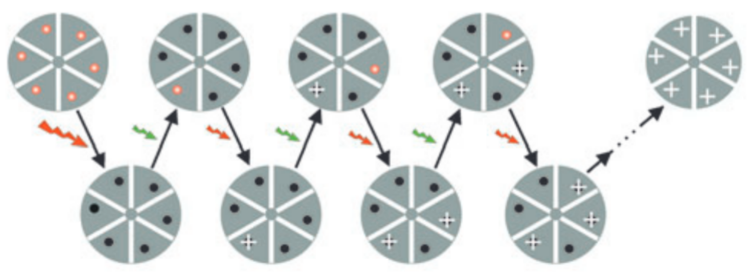
\includegraphics[width=0.5\textwidth]{figs/photoswitchStorm.png}
	\caption{STORM imaging sequence, taken from \cite{rust2006sub}. For demonstration, Rust et al. present a hypothetical hexameric object containing red fluorophores. In the first instance, a powerful red laser is used to turn all of the fluorophores into the dark state. In the second, a green laser pulse is used to activate some fraction of the fluorophores, sending them to the emitting state. Illumination from a red laser then stimulates emission from these fluorophores until they are switched off. The white crosses denote molecule positions which have been determined to high accuracy. The overall image is constructed from the amalgamation of many different imaging cycles.}
	\label{photoswitchStorm}
\end{figure}
%/home/seanbaccas/Documents/maths/MSC/MScProject/maybeClustering/writeUp/moreLit/cyanine dye paper

The raw SMLM data consist of roughly 10,000 frames are captured over a square field of view which, in this case, is 127$\mu$m wide. Images are then turned into a table of \textit{localisations}, which is essentially a list of the coordinates of the identified fluorescent molecules (fluorophores), alongside with some other characteristics, such as the estimated uncertainty in the measure of these coordinates. There are a variety of software packages availabe for this procedure, such as ThunderSTORM \cite{thunderstorm}.
% In brief, it's a software tool that allows for the reconstruction of super-resolved images. It can be used to set a minimum signal-to-noise threshold, so that imprecise localisations are removed\footnote{later, discuss how we can improve their read-in with GPUs.}.




% They state that the aforementioned Cy5 or Alex Fluor 647\footnote{\textbf{cite}} are the best available fluorophores for \textit{direct STORM}\footnote{When only a single dye is used, see van de Linde et al., 2011 from this paper}, due to their high photon counts, desirable blinking properties\footnote{Which are?} and high photon counts. \textbf{State also that these dyes can go through many cycles before bleaching occurs.} \\

% \textbf{stuff to note:}
% \begin{itemize}
% 	\item fiducial markers are used to correct sample drift.
% 	\item why don't they all get lit up at once?
% \end{itemize}

% \subsubsection{Image reconstruction}
% \textbf{todo - see paper in comment}\\
% %https://aip.scitation.org/doi/pdf/10.1063/5.0069349
% Below follows some notes on the "image reconstruction" chapter of \cite{stormAndThunderstorm}.\\



\subsection{The Issues Encountered When Attempting to Process Point Cloud Data}
% \textbf{todo:}
% \begin{itemize}
% 	\item attempt to quantify the difference in scales we're looking at here
% 	\item discuss the effect of imaging artefacts - note that our method includes the standard deviation from the read-in section as well 
% \end{itemize}
% \textbf{stuff to mention}
% \begin{itemize}
% 	\item the output is a point cloud of x and y coordinates
% 	\item we want to evaluate the cluster proposals
% 	\item \cite{19FromKhaterEtAl} talks about why we care about clustering
% \end{itemize}


Having discussed SMLM, we turn our attention now to the problem of quantifying the data that we receive from SMLM processes. Much of the following chapter will follow \cite{Lelek2021}, which is a comprehensive review of the cluster analysis and quantification methods. As mentioned by the authors, the majority of methods are based on second-order statistics\cite{Lelek2021}, which are sensitive to noise and imaging artefacts. This review also discusses localisations in three dimensions.  \\

Broadly speaking, the analysis of the size, location and other characteristics of clusters allows for the extraction of a signature of the underlying biological processes. Indeed, as Pageon et al. \cite{clusterDetection} put it, SMLM techniques retain spatial information of each molecule, allowing for granular access to local parameters to establish hierarchical information at various scales, be it at the level of the entire cell, at the level of protein clusters, or at the level of molecules\cite{clusterDetection}. Much of the methods in this space relate to protein-protein interactions, and understanding the structure and organisation of their clusters is crucial to understand how they function within the cell \cite{Khater2020}. Figure \ref{fig5FromKhater} (from \cite{Khater2020}) motivates the need to quantify the clusters within biological samples, as this understanding is important to differentiate between the various \textbf{paths} that a system may take from one state to the next.\\



%The advent of SMLM has caused a large shift in the data extracted from the imaging \textbf{process}. Rather than \textbf{wide-field, unfocused} images, the data are now precise point-clouds indicating the localised position of every molecule that could be seen to fluoresce throughout \textbf{the imaging time}. \\

%talk about the paper we saw as a reference in 19 from khater
%file:///home/seanbaccas/Documents/maths/MSC/MScProject/maybeClustering/writeUp/moreLit/reviewLipidInsight.pdf
The review from Owen et al. \cite{lipidRaftHypothesis} details some of the important insights that it was possible to garner with this order-of-magnitude improvement in imaging resolution. When discussinglipid rafts, the most accurate description that could be given about them was one that referred to their small and dynamic nature. Whilst their importance in cellular processes was appreciated, the methodologies used to study them were inherently limited by diffraction-limited microscopy \cite{lipidRaftHypothesis}. The advent of SMLM methods, such as PALM \cite{shroff2013photoactivated} and STORM \cite{rust2006sub} then allowed this definition to be updated to reflect that small perturbations can easily tip the balance between cell systems settling in different configurations \cite{lipidRaftHypothesis}, c.f. \cite{25FromLipidRaft}. Moreover, these new super-resolved imaging methods allow for much deeper insights into the ultimate function of rafts, regulating the distribution and diffusion of membrane associated proteins, as well as regulating protein interactions for efficient signalling and trafficking \cite{lipidRaftHypothesis}. It is with processes like this in mind that we interest ourselves in the clustering of molecules within biological systems.\\

The problem now is to efficiently analyse the pointillist data that comes out of static-cell imaging processes like STORM. This representation is fundamentally different to those used in conventional microscopy, namely the intensity grid valued pixel and voxel image representations \cite{Khater2020}. These representations are challenging to perform inference upon, largely due to the quantisation errors that may be introduced during the voxelisation, but more broadly analysing them can be challenging to due the sparse nature of their representation \cite{s21165574,s21248241}. The granular nature of point cloud data can provide much deeper insights, but needs newer, bespoke analysis tools. Identifying and characterising the clusters of fluorophores are the most suitable way to gain insight into SMLM data \cite{Khater2020}. \\

The field of cluster analysis is a well-researched topic in computer science is detailed and well-studied. Please refer to \cite{jain1999data} for a review. The main issue that we encounter when trying to cluster data is the combinatoric complexity, as well as the issue of the assumptions that must be made when deciding what constitutes membership of a cluster. Ideally, the method used should rely on as few priors and user-defined parameters as possible. The data in this context are unlabelled, meaning that the clusters must be elucidated purely from the spatial distribution of the points within them.

\subsubsection{The images in question}
Of particular interest of this project is the imaging of nucleosomes and related protein complexes. DNA consists of billions of individual base pairs that express genes, which would stretch to over a metre if laid out in full. When in the nucleus, these base pairs are wrapped around approximately 30 million nucleosomes, forming a complex called chromatin \cite{xu2019guide, flavahan2017epigenetic}. The compacted DNA can be reduced in length by six orders of magnitude, so that it can fit within the nucleus of a cell. Whilst the DNA sequence is fixed, the structure of chromatin is constantly in flux due to a wide range of processes \cite{xu2019guide}. Modern advances in microscopy techniques have been very fruitful for uncovering the dynamics of higher-order chromatin structure in a variety of biological processes \cite{xu2019guide}. In particular, Xu et al \cite{xu2022ultrastructural} went on to demonstrate various direct clinical uses for imaging chromatin structure, as they showed its shape is disrupted as cells undergo carcinogenesis. 
Furthermore, Ricci et al \cite{ricci2015chromatin} showed that nucleosomes group together in groups of various sizes, and that the density of their groups was specific to each cell-type. In other words, the \textit{clusters} of various biological cells are important in understanding what occurs at the cellular level, and the advent of SMLM has played a key role in enabling our understanding of such processes.
%time to discuss ricci et al -- distribution of dna in the nucleus is characteristic between different cell types

\section{What algorithms are there for performing cluster analysis?}

%in \cite{55FromKhater} they claim that the bayesian paper we observe is the first one. could we think of improvements?
As mentioned, the topic of identifying clusters is a well-studied one in computer science. For this section, we will discuss the problem at hand, as well as many of the most popular methods for identifying and quantifying SMLM clusters, following on from \cite{Khater2020}. \\

The output data from ThunderSTORM is a large list of \textit{localisations} with associated metadata. Each localisation consists of $x$ and $y$ coordinates of the fluorophore within the FOV, as well as the frame number in which this photon was detected, the number of photons detected in this position, and the uncertainty in the position of each of the coordinates, which will become  important when we come to discussing the Bayesian algorithm in section \ref{bayesianClusteringAlgorithm}. Also included is the width of the point spread function that produced the given photon, which we can use to remove erroneous data from the localisation table. We expect the PSFs produced by Alexa 647 in STORM imaging to be between 160 and 200nm\cite{thunderstorm}, meaning entries outside of this range can be chalked up to artefacts of the imaging or localisation process. In some instances we will observe phantom clusters produced by particular fluorophores blinking in multiple frames - we can use the photon count measure to correct for this. \\

Identifying the clusters in a (typically very large) dataset is a problem which seeks to determine groups of molecules which appear to be more densely packed than the image in general. 
As we shall discuss in depth when outlining the Bayesian method for identifying clusters, this can come down to selecting a spatial scale at which the localisations can be considered \textit{clustered}. 
Getis and Franklin \cite{getisAndFranklin} summarise the relationship of localisation $i$ with all the other $j \neq i $ as being represented by the distance between $i$ and all of its neighbours and the spatial scale at which the local density of localisations appears different from the global density. This method identifies clusters by determining a scale at which we consider clusters to be statistically significant. We begin by discussing statistical methods of determining clusters.\\

\subsection{Statistical Methods} \label{statisticalMethods}

Ripley's K function \cite{ripley1977modelling}, as well as similar measures named after him, are popular methods for identifying clusters. Prior to this work, spatial patterns were usually identified by testing the likelihood that a particular pattern could have simply been generated by a random process, such as the Poisson process. Ripley's method was built on the assumption that a full map of the spatial pattern was available (as is more or less the case when dealing with SMLM data), searching for \textit{second-order} methods to test whether a pattern is different from random noise. We call this a second-order method since it concerns second moment properties: the first moment property is simply the number of localisations in a given area, whereas the second moment relates to the expected number of localisations within a fixed distance of another point \cite{kiskowski2009use, Khater2020}. We define Ripley's K function here, since it is important background for how we determine clusters at a later stage. Formally it is defined as \cite{ripley1977modelling, kiskowski2009use}:

\begin{equation*}
	K(r) = \frac{1}{n} \sum_{i = 1}^{n} N_{p_i}(r) / \lambda,
\end{equation*}

where the sum is taken over all $n$ points in the dataset, and $N_{p_i}(r)$ is the number of points within a distance $r$ of $p_i$. We have also that our score is normalised by the number of points per area $\lambda$. The expected value of $K(r)$ for a random distribution, generated by the Poisson process, is $\pi r^2$ \cite{kiskowski2009use}. The reason for this is that a uniformly random distribution of points will have $N_{p_i}(r) = N_{p_j}(r) = n$, meaning that, replacing $\lambda = \frac{n}{\pi r^2}$, summing from 1 to $n$ will yield $\frac{1}{n} \cdot n^2 \cdot \frac{\pi r^2}{n} = \pi r^2$. We can then use this to measure clustering: $K(r) > \pi r^2$ indicate regions of higher density than a uniform background.\\

\subsubsection{One Method In Particular} \label{GandFdiscussion}

It was this idea of analysing the densities around each point that led to the formation of the analysis technique which we focus on in this project. The method from Getis and Franklin \cite{getisAndFranklin} was developed following their technique to describe the tree spatial patterns at a number of scales. Developed following Ripley \cite{ripley1977modelling}, their analysis is designed to test randomness hypotheses, by examining the proportion of pairs whose members are within a certain distance of each other\cite{getisAndFranklin,ripley1977modelling}. They state that these methods are similar to second order analysis, but rather than producing a measure for the whole dataset, instead focusing on issuing a score for each point $i$ individually. They define the score for each point as follows \cite{getisAndFranklin}:

\begin{equation*}
	L(r)_i = \sqrt{A \sum_{j = 1}^{N} \frac{\delta_{ij}}{\pi(N-1)} },
\end{equation*}
where:

\begin{equation*}
	\delta_{ij} =
	\begin{cases*}
		1 & if $i \neq j$ \ \text{and} \ $|i - j| \leq r$ \\
		0 & otherwise
	\end{cases*}
\end{equation*}
Here $A$ is simply the area of the ROI.	
They include also an edge-correction for when the distance $r > |i - j| > e_1 $, with $e_1$ being the distance to the nearest boundary. In this case, $\delta_{ij}$ takes the value:

\begin{equation}
\label{edgecorrection}
	\frac{1}{1 - \arccos(e_1 / r) \frac{1}{\pi}},
\end{equation}  

which is at least 1 and is maximised the closer point $i$ is to the edge of the ROI. If $i$ is closer to \textit{both} boundaries than to point $j$, then $\delta_{ij}$ takes the value:

\begin{equation*}
	\frac{1}{1 - \frac{1}{2\pi} ( \arccos(e_1/r) + \arccos(e_2 / r) + \pi / 2 )},
\end{equation*}

where $e_2$ is the distance from the point $i$ to the other boundary. This allows us to still compute the score for a point, where additional contributions may be obscured by the boundary of the ROI.\\

We have here, inspired by Getis and Franklin \cite{getisAndFranklin}, reproduced some diagrams that illustrate the usefulness of their measure. In figure \ref{randomScatterFigs}(a), we have highlighted a central point, surrounded by a sea of randomly scattered others. Figure \ref{randomScatterFigs}(b) demonstrates that, as we increase $r$, gradually more and more points come within a distance $r$ of our central point, leading to $L(r)$ increasing. Due to the points being scattered randomly, we expect the sum total of the number of points within a distance $r$ to be proportional to the area of our scan, $\pi r^2$. The $\pi$ and the square root were explicitly chosen so that $L(r)$ would be \textit{linear} in $r$, as we can see when compared with a straight line of best fit. \\

Figure \ref{NRscatterFigs} shows a perhaps unwieldy, but still useful complementary example. Our highlighted central point is now isolated from a dense region of other points by about 0.15 units. This is reflected in the graph of $L(r)$ against $r$: it remains at 0 until the first member of the cluster comes within range, before rapidly picking up. This steep gradient here, in their words, implies a tendency for clustering \cite{getisAndFranklin}. At just under 0.2 units, $L(r)$ passes above the linear line, meaning that we now have denser clustering than a uniform, spatially random background. We see further that the curve peaks and levels off at just under 0.3 units, showing us that the clustering is saturated. The authors give also some reasonable numbers for the $y$ - intercept on such a straight line of best fit, that would represent the 5\% and 1\% line of best fit, namely $\pm 1.42 \sqrt(A)/(n-1)$ and $\pm 1.68 \sqrt(A)/(n-1)$. Herein lies the issue that this measure aims to solve: when viewed at a scaled of 0.1 units, the isolated large dot in figure \ref{NRscatterFigs}(a) appears distinct from the other points. If we instead zoom out and observe at a much larger scale, all the points in this smaller ROI could be considered part of the same cluster. So, which scale do we choose?\\

Getis and Franklin \cite{getisAndFranklin} state that the variance about the observed mean $\bar{L_i}(r)$ for a particular $r$ indicates how much clustering occurs within a particular pattern, and that the greatest contrast in pattern will be seen when the variance of $L_i$ is maximised. In figure \ref{variances}, we demonstrate this, with our curve showing two distinct peaks, one indicating maximal clustering as $r$ becomes large enough for the three individual clusters to be self-contained, and finally a second peak as $r$ becomes large enough that the all of the data are drawn into one cluster. Part of selecting a scale is some prior understanding of the data itself: whilst the largest variance we see in figure \ref{variances} is for a value of $r$ that is large enough to mean that all three of the other clusters are within reach of the enlarged point of interest, indicating that all of these points belong to the same cluster, it would be reasonable to impose some kind of maximum value on $r$, as we may consider that it makes little sense for all these (seemingly distinct) groups of points to be regarded as part of the same cluster.
This tool from Getis and Franklin is a useful tool for indicating interesting values of $r$ where the nature of the clustering seems significant, which we shall revisit when discussing its use in the context of biological clusters. Whilst Ripley's K function can provide insight into the global structure of the data, Getis and Franklin's function provides insight into each localisation \cite{Khater2020}. 

\begin{figure}[t!]
\raggedleft
	\subfloat[\centering Random, uniformly distributed background, with one central point (enlarged for clarity). ]{{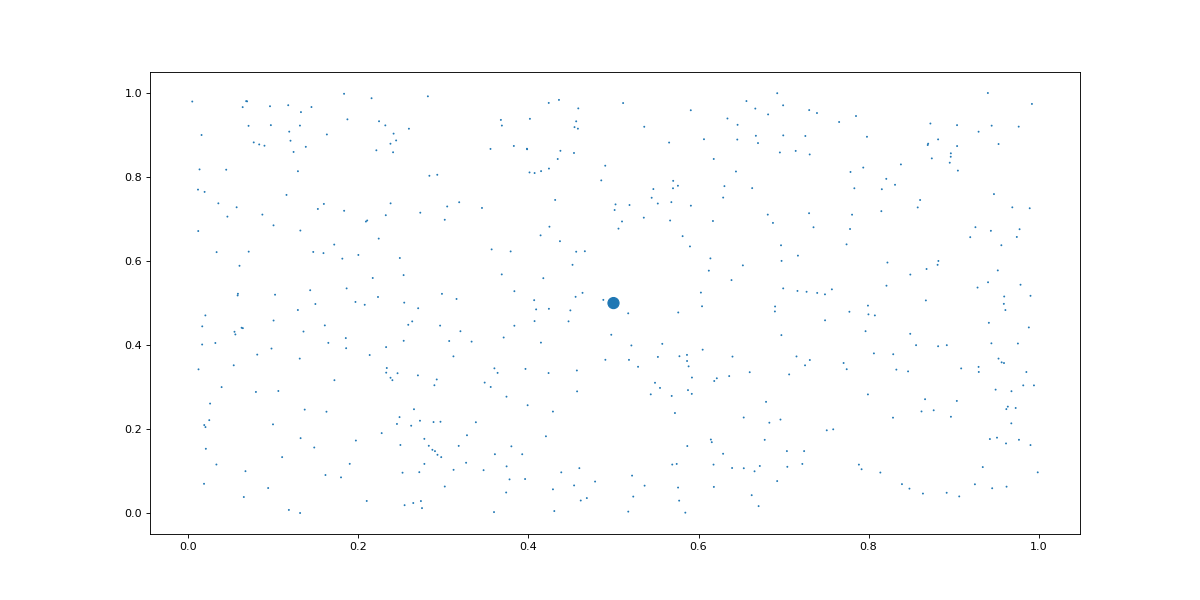
\includegraphics[width=0.9\textwidth]{secondOrderExperiment/scatter.png} }}
	\qquad
	\subfloat[\centering Graphs of $L(r)$ against $r$, where $r$ is taken to be the distance from our central point at coordinates (0.5,0.5). The second graph includes a linear line of best fit. ]{{\raggedleft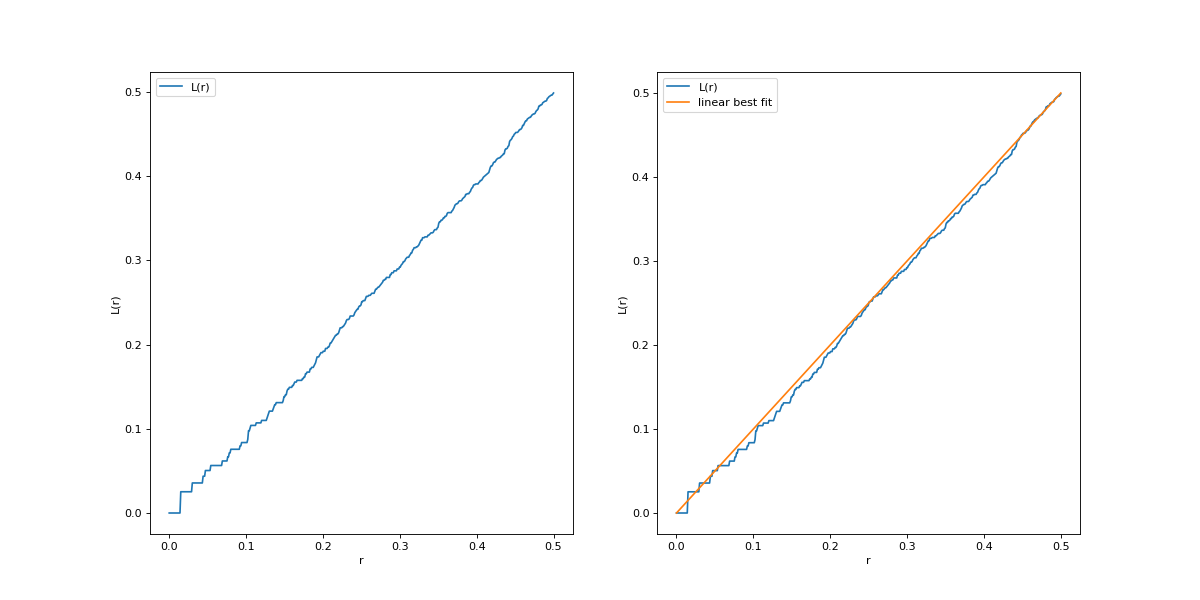
\includegraphics[width=1.1\textwidth]{secondOrderExperiment/lrAgainstR.png} }}\hfil\label{pixelShift}
 	\caption{This figure demonstrates the \textit{linearity} of localisation score against distance for the enlarged point in the centre of figure (a). We see this linearity due to the fact that the background process is uniformly random in all directions. Alongside figure (b) is a linear line of best fit. }%
	\label{randomScatterFigs}%
\end{figure}
%\section{Why do we care about clusters? What are the implications?}

\begin{figure}[t!]
	\centering
	\subfloat[\centering In the bottom left we have an enlarged point of focus, this time isolated from a large group of other points ]{{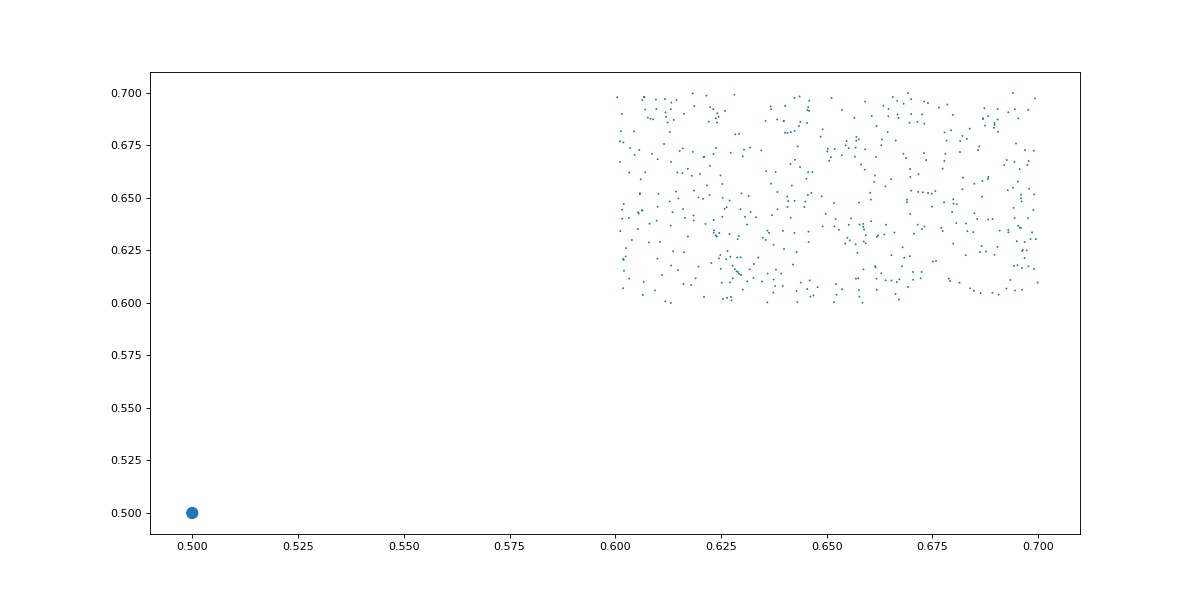
\includegraphics[width=0.9\textwidth]{secondOrderExperiment/scatterNR.png} }}
	\qquad
	\subfloat[\centering These graphs depict $L(r)$ against $r$ for the situation in figure(a). The line remains flat for approximately 0.14 units, as there are no other points within this distance of the bottom left corner. As $r$ increases, the large cluster in the top right corner of figure (a) suddenly come within reach, causing $L(r)$ to jump upwards. ]{{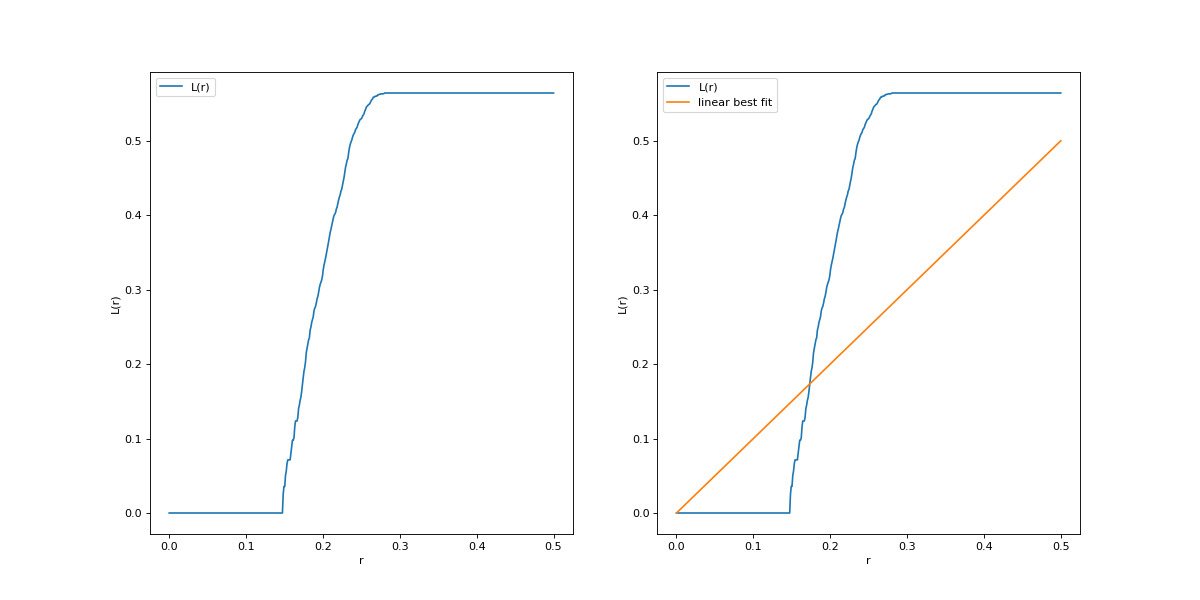
\includegraphics[width=1.11\textwidth]{secondOrderExperiment/lrAgainstRNR.png} }}
	\caption{Recreation of the scenario in figure \ref{randomScatterFigs}, except that our point of interest is no longer surrounded by a uniform background, instead by a large group of other points, approximately 0.14 units away. This causes a large change in the localisation score for the point of interest }%
	\label{NRscatterFigs}
\end{figure}

\begin{figure}[t!]
	\centering
	\subfloat[\centering A similar situation to figures \ref{randomScatterFigs} and \ref{NRscatterFigs}, except with a distinct point separated from three clusters.]{{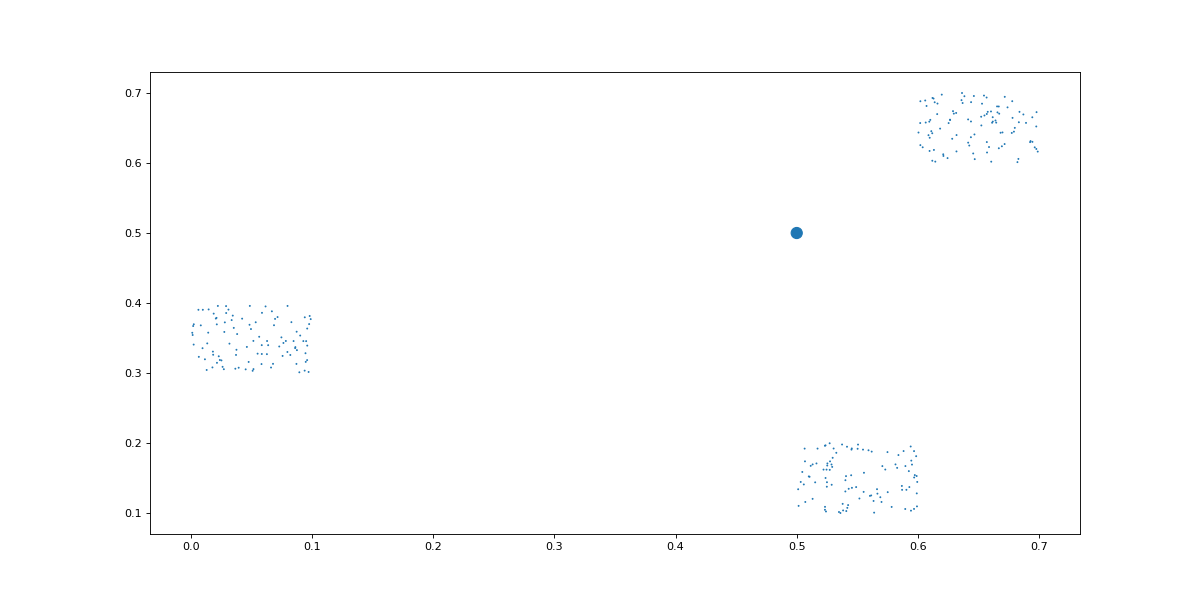
\includegraphics[width=0.6\textwidth]{secondOrderExperiment/bigscatter.png} }}
	\qquad
	\subfloat[\centering For each $r$, we calculate the $L_i(r)$ for each point $i$ in the data, and plot the variance of these values against radii. We see two peaks, as the large variance in the scores indicates firstly that we have local clustering, as $r$ becomes large enough for each of the points within the clusters to detect all of each other, and secondly that we have clustering on a global scale.  ]{{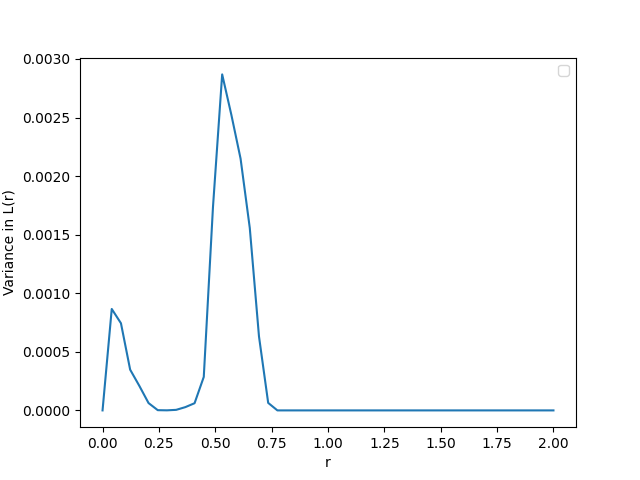
\includegraphics[width=0.6\textwidth]{secondOrderExperiment/variances.png} }}
	\caption{This figure shows a slightly altered situation relative to figures \ref{randomScatterFigs} and \ref{NRscatterFigs}, this time with plots of the variances in all of the $L_i(r)$ values for each point in the data. }%
	\label{variances}
\end{figure}


% \begin{figure}[t!] 
% 	\centering
% 	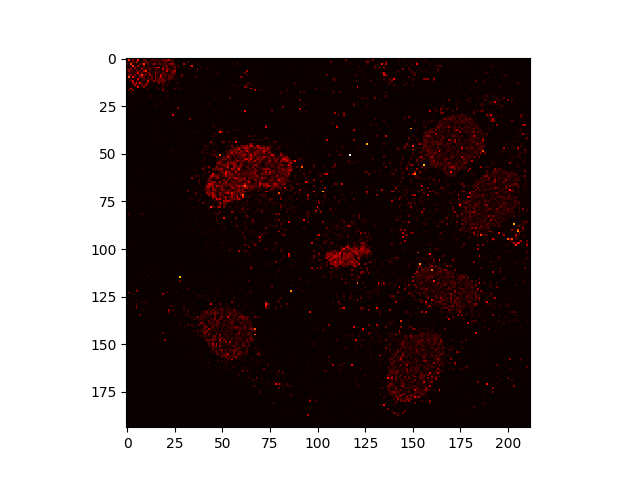
\includegraphics[width=0.5\textwidth]{figs/1_un_red_csv_raw.png}
% 	\caption{Low-resolution scan of \textbf{1\_un\_red.csv} }
% 	\label{1_un_red_csv_raw}
% \end{figure}

\begin{figure}[t!] 
	\centering
	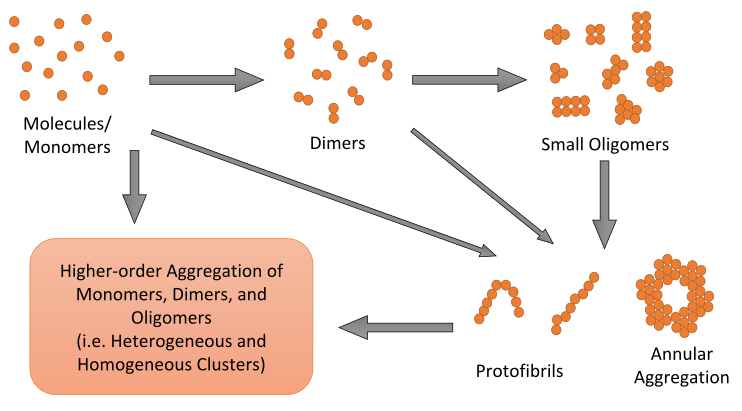
\includegraphics[width=0.5\textwidth]{figs/fig5FromKhater.png}
	\caption{This figure appears as Figure 5 in \cite{Khater2020}. It demonstrates how individual molecules can either directly form larger, more complicated structures, or perhaps go through a long chain of other processes. The analysis of the molecule clusters can provide insight into the nature of the process at hand. }
	\label{fig5FromKhater}
\end{figure}



% \subsection{Other Noteworthy Clustering Methods}

The goal of this project was to demonstrate it was possible to efficiently implement the above cluster proposal mechanism, combined with the Bayesian evaluation method outlined in section \ref{themodelitself}, to create a scalable method for processing SMLM data. For details on other methods, we refer the reader to \cite{Lelek2021}.





\section{Bayesian Clustering Algorithm} \label{bayesianClusteringAlgorithm}

% \textbf{TODO}
% \begin{itemize}
% 	\item discuss Dirichlet process (see their citation number 26 in the paper)
% 	\item not sure the dirichlet process is too important - better use of time would be discussing getis and franklin.
% 	\item how good is our model? why is it gaussian spread from the centre? see the wiki page for airy disc - we can produce a curve to show they match each other closely
% 	\item mention each localisation gets its own error from the localisation process
% 	\item essentially we draw up proposals using the second order nbhd of mapped points, and then rate them for how closely they conform to a gaussian
% \end{itemize}

In this section, we will present the methodology described by Rubin-Delanchy et al. \cite{Rubin-Delanchy2015}, and go on to describe how it has been implemented in our repository. The process has two stages: cluster generation and cluster evaluation. It should be noted that the main contribution of \cite{Rubin-Delanchy2015} is a model for what the ideal cluster should look like, and a way of assessing how closely the proposed clusters conform to that model. This part of the process is agnostic towards the cluster-generation procedure, and many of the methods discussed earlier would also be suitable. \\

The model for the data makes a few key assumptions. Firstly, the localisation process is assumed to disturb by the true positions of the molecules by errors which are Gaussian-distributed. Each localisation $i$ has its own standard deviation value (which we denote $s_i$), estimated on the basis of of the number of collected photons, PSF width, local background noise and camera pixel size \cite{Rubin-Delanchy2015, 25fromRubinDelanchy}.
Secondly, the clusters themselves are assumed to be uniformly distributed across the ROI, against a completely spatially random (CSR) background, with a probability distribution for their radii being supplied by the user. This distribution should be specific to the situation being imaged, and we give a discussion on this in section \ref{sigmacurvediscussion}.\\
%The main contribution of this method is the computation of posterior probabilities of cluster assignment, given the above model. 

Before we begin, we outline some of the terminology and definitions that will be used going forward.
\begin{itemize}
	\item \textit{Localisation} - localisations are assumed coordinates for a molecule. In the scope of this report, a localisation $i$ will be characterised by its central coordinates in two dimensions, $V_i = (x_i, y_i)$. Each localisation is assumed to be disturbed from its true molecule position $Z_i$ by an error which is Gaussian-distributed. The standard deviation from its centre is labelled $s_i$.
	\item $\theta_k = (\mu_k, \sigma_k)$ - for a given cluster $k$, these are respectively the assumed central coordinates and radius of the cluster.
	\item $L_i(r)$ - this is the localisation score for each localisation $i$, as discussed in section \ref{GandFdiscussion}.
	\item $R$ - this is one of the two main parameters we vary when drawing cluster proposals. As we shall see, we determine that any two localisations which are (a) not members of the background and (b) within a distance 2$R$ of each other, are members of the same cluster
	\item $T$ - this is the other main parameter we vary. In each round of cluster proposal generation, any localisation whose score $L_i(R)$ is below this threshold $T$ are determined to be members of the background.
	\item \textit{Complete Spatial Randomness (CSR)} - CSR is our reference for a typical, un-clustered, uniformly distributed background. Its definition is a background generated by the Poisson point process \cite{getisAndFranklin}, and we draw cluster proposals by comparing with CSR. 

\end{itemize}

\subsection{Generation of Cluster Proposals}
%The cluster proposals are generated with a method based on Ripley's K function \cite{ripley1977modelling}.

To generate the cluster proposals, we need to define what it means for any individual localisation to be a member of a cluster, and what it means for two localisations to be part of the same cluster.
% We model our data to be a set of Gaussian clusters, laid over a completely spatially random (CSR) background \cite{Rubin-Delanchy2015}. This means that 



\subsubsection{Localisation Score} \label{localisationScore}

%The first step is to calculate a clustering score $L_i$ for each point $i$ in the set of localisations. This score was proposed by Getis and Franklin \cite{getisAndFranklin}\footnote{TODO - discuss why they made this and what it's good for.}. For each localisation $V_i$, its localisation score is calculated as:

The generation of cluster proposals is based on the localisation-scoring of Getis and Franklin \cite{getisAndFranklin}, as detailed in section \ref{GandFdiscussion}. We build on this, and discuss how clusters are drawn from there.\\


%At this stage, the authors of \cite{Rubin-Delanchy2015} incremented values of $r$ from 5nm to 200nm to \textbf{give a variety of reasonable values for this prior}. The upper limit of 200nm is chosen since conventional microscopy are resolvable above this \textbf{range}\footnote{I think we use only one value for this - which is it?}. \\

For each localisation $i$, this $L_i(r)$ is a function of the number of other localisations within a distance $r$ of $V_i$, normalised by the total number of pairings where our localisation of interest is one of the members, $N-1$.  The value of $r$ is incremented from 5nm up to 200nm. This upper limit is chosen since any clusters larger than 200nm are resolvable with standard fluorescence microscopy\cite{Rubin-Delanchy2015}. Here the constant $A$ represents the area of the (rectangular) ROI. In our implementation of this algorithm (see section \ref{algImplementation}), the ROI is scaled down to a square with side length of 2 units. \\

After this score is calculated for each localisation in the dataset, any points which have $L_i < T$, for some threshold $T$, are determined to be background points. This is because for this value of $r$, the localisation $i$ is determined to be in a region that is insufficiently dense to be part of a cluster. The idea behind this method is to compare the density around each localisation with the density expected under CSR. As such, we would expect that $L(r)_i$ being less than $r$ would indicate points that are less clustered than under CSR \cite{Rubin-Delanchy2015}. This is by design: as demonstrated in section \ref{GandFdiscussion}, we see that $L_i(r)$ is linear in $r$ for a localisation amongst a CSR background. \\

%\textbf{Why do we choose this method for generating the localisation proposals?} Firstly, this score is very easy to compute, and can be enhanced with the use of polar coordinates (see section \ref{algImplementation} for details). Secondly, this localisation score is crucial to establishing a sensible scale at which we can consider the individual molecules to be part of some cluster. \textbf{mention more from getis and franklin, perhaps include their figure. importantly it picks out when we are suddenly matching the background process. The distance chosen represents the scale at which one can view the pattern -- i think the point is since we use the bayesian scoring anyway it doesn't matter}

This method for generating proposals was chosen for a number of reasons. Firstly, the score itself is very easy to compute, as for each localisation $i$, the calculation involves little more than counting its nearest neighbours, and then multiplying by a constant scaling factor. As we shall see in section \ref{algImplementation}, there are a various ways upon which this can be improved in its implementation. Secondly, this method is agnostic to the scale at which the ROI is being viewed. It's worth reiterating that any cluster-proposal method can be used at this stage of the process, but the low computational cost of this method is attractive, given that we intend to analyse a large number of them to determine the proposals that fit closest to the model we outline in section \ref{thebayesianmodel}.


%To see this, let us examine the localisation score as $r$ tends towards infinity:
%
%\begin{equation*}
%	L(\infty)_i = \sqrt{\frac{A}{\pi (N-1)} \sum_{j = 1}^{N} \delta_{ij}}
%	= \sqrt{\frac{A}{\pi}}
%\end{equation*}
%
%In particular, 


\subsubsection{Cluster Radius}
We say further that for some \textit{clustering radius} $R$, that two localisations with coordinates $V_i$ and $V_j$ are members of the same cluster when their separation $|V_i - V_j|$ is less than 2$R$. 


This way of assigning molecules either to (a) the background or (b) some cluster, will assign every datum to a cluster of size at least 2, or to the background. To see this,
we fix a value for $R$ and $T$, and let $V_i = (x_i, y_i)$ be a localisation such that $|V_i - V_j| < R$, $\forall j \neq i$. Hence we have that $L(R)_i = 0$, meaning that this $V_i$ is determined to be a member of the background process for all $T > 0$. If we change this so that there is exactly one $V_j$ within a distance $R$ of $V_i$ (and vice versa), then (taking the area $A = 4$) we have that these two points are either members of the same cluster (of size 2) or are both background points $\forall \ T > \sqrt{\frac{4}{\pi(N-1)}}$. \\


\subsection{The Bayesian Model}
\label{thebayesianmodel}

As mentioned above, the main contribution of the authors of \cite{Rubin-Delanchy2015} is the calculation of posterior probabilities. More specifically, once  proposed set of clusters has been generated for a value of the parameters $R$ and $T$, we can determine the likelihood that each point in the dataset would have been given its label, based on the supplied parameters. In this subsection, we'll dive into exactly how this is calculated. 

\subsubsection{Preliminaries}
We begin by describing the dataset. The data are a vector of $N$ different localisations $V_i$. Each of these carry an associated variance $s_i^2$, which denote the error introduced at the time of localisation, as mentioned in at the beginning of this chapter. 
We aim to create a vector $L = [l_i, \ i = 1, \dots , N]$ of $N$ different labels, each one denoting membership to a particular cluster. If $l_i = l_j$, then the localisations $i$ and $j$ at coordinates $V_i$ and $V_j$ are part of the same cluster. We reserve the label $l_i = 0$ to denote that localisation $i$ is part of the background. In general, if we identify $m$ clusters, we should then have $l_i \in \{0, 1, \dots, m\}$, i.e. $m+1$ distinct labels. Furthermore, for a cluster $k$, let $c_k$ denote the set of localisations $i$ that are a member of cluster $k$, and $n_k$ be the cardinality of $c_k$. In particular, if some localisation $j$ is a member of cluster $k$, then we have that the label $l_j = k $. As we shall see, the most crucial part of this process is calculating, for a proposed set of labels $L$, and a given vector of localisations $\nu = [V_i, \ i = 1, \dots, N]$, the calculation of $p(L|\nu)$. We interpret this as the probability of observing a set of labels, given the known set of localisations. It is this measure which determines the quality of a proposed set of clusters, and herein we shall refer to it as the \textit{posterior probability}.  \\

\subsubsection{The Model itself}
\label{themodelitself}

We now can describe the model of \cite{Rubin-Delanchy2015} in more detail. Our aim here is, given a proposed set of labels $L$ (determining which localisations have been determined to be part of the same cluster, and which are background points), to establish how \textit{likely} it is to observe this set of labels, given a model for forming clusters. We begin by noting a few key assumptions. As mentioned before, we assume that the coordinates $V_i$ of each localisation $i$ are disturbed from the true molecule position $Z_i$ by a Gaussian-distributed error, with its standard deviation being labelled here as $s_i$. Further to this, we have that each \textit{cluster} is modelled as a Gaussian: for some cluster with label $k$, we assume that all of the true molecule positions that are located in this cluster are distributed around the cluster centre $\mu_k$ with standard deviation $\sigma_k$. More specifically, we have that $Z_i ~\sim \mathcal{N}(\mu_k, \sigma_k^2 I_2) $, where $I_2$ is the two-dimensional identity matrix. With these two assumptions, combined with a linearity argument, we can say that we should expect that a localisation $i$ with position $V_i$ will satisfy:

\begin{equation}
	\label{VDistribution}
V_i ~\sim \mathcal{N}(\mu_k, (\sigma_k^2 + s_i^2) I_2).
\end{equation}

The two standard deviations have been added together, encapsulating the Gaussian shape of the cluster and the nature of the assumed localisation errors. \\


Our aim, as mentioned above, is to calculate $p(L|\nu)$ which, by Bayes' theorem, we can state is proportional to $p(L)P(\nu|L)$, the probability that we have some set of labels, multiplied by the probability that we have a particular set of localisations given a set of labels. As we shall outline, these two quantities can be calculated, but not necessarily in a closed analytic form. The authors of \cite{Rubin-Delanchy2015}, following on from the work of \cite{10.1214/aos/1176342360}, give an expression for the probability (density) that a certain labels will be issued, given the number of points in some cluster, the number of identified clusters, and the number of background points. This measure was developed through the Dirichlet process, which aims to establish some prior knowledge of the distribution of random variables. We quote the result here, from \cite{Rubin-Delanchy2015}:
%Points which are determined to be part of \textit{some} cluster through their localisation score are then grouped using the \textbf{Dirichlet process}, with one important hyperparameter $\alpha$, called a concentration parameter\footnote{TODO: discuss the concentration parameter}. Then, following Green and Richardson \cite{greenAndRichardson, Rubin-Delanchy2015}\footnote{TODO: discuss this paper fully}, a proposed labelling for all $N$ localisations $l$ has the prior probability:



%essentially the dirichlet process, beyond the scope of this report, attempts to a assert a meaningful probability distribution for a some random variables.

\begin{equation} \label{priorProbability}
	p(L) = p_B^{n_0} (1-p_B)^{N - n_0} \frac{\alpha^m \Gamma(\alpha) \prod_{k = 1}^m \Gamma(n_k)
											}{\Gamma(\alpha + N - n_0)
										},
\end{equation}
where $n_k$ denotes the number of points in cluster $k$ (with $k=0$ denoting the background points). The hyperparameter $\alpha$ is known as the concentration parameter \cite{Rubin-Delanchy2015}. The sensitivity of the algorithm to this parameter is yet to be established. \\

At this stage, we should note a few key details, following \cite{Rubin-Delanchy2015}. Firstly, 
clusters are \textit{independent} of each other, meaning the likelihood that some cluster $k$ has parameters $\theta_k$ is independent of any of the other cluster parameters. Secondly, the points within a cluster are identically distributed in a Gaussian pattern around the cluster centre, as described above. Thirdly, background points are uniformly distributed across the ROI. We shall add some clarifications to these points after introducing some more elements of the model.\\ 

%We have further that all clusters $k \geq 1$ contain points which are distributed in a circular Gaussian pattern with unknown\footnote{expand on why this is unknown at compute time} mean (centre coordinates) and variance (a proxy for radius). More concretely, for $i \in c_k$, then the true molecule centre $Z_i$\footnote{associated with localisation $V_i$} will satisfy $Z_i ~\sim \mathcal{N}(\mu_k, \sigma_k^2 I_2) $. We have that $\mu_k$ is uniformly spread across the region, whereas a sensible cluster width must be supplied by the user\footnote{TODO: add a section where we discuss the specifics of the experiment at hand}. \\

With all of this, and Bayes' theorem, we can calculate the probability (density) that we would issue a certain set of labels $L = [l_1, l_2, \dots]$, given the set of localisations observed $\nu = [V_1, V_2, \dots]$. In particular, since $p(L|\nu) \propto p(L)p(\nu|L)$, we can state that \cite{Rubin-Delanchy2015}:

\begin{equation} \label{probLGivenV}
	p(L|\nu) \propto p(L) \Bigg[
			\underset{i \in c_0}{\prod} p_0(V_i) \cdot
			\overset{m}{\underset{k = 1}{\prod}}\int p(\theta_k)
			\underset{i \in c_k}{\prod}p(V_i | \theta_k) d\theta_k
%			
	\Bigg]
\end{equation}


It's useful at this stage to discuss the meaning of each the terms in the expression $ p(\nu|L)$. Firstly, $\theta_k = (\mu_k, \sigma_k)$ are the parameters\footnote{Central coordinates and cluster radius.} associated with cluster $k$. Given that we expect clusters to be uniformly distributed across the ROI, we take $p(\theta_k) = p(\mu_k)p(\sigma_k) = \frac{1}{A}p(\sigma_k)$.
$p_0(V_i)$ refers to the background probability density, meaning the probability that some localisation at position $V_i$ was is a member of the background. Since we assume that background points are uniformly distributed across the ROI, we can state that $p_0(V_i) = 1 / A$, where $A$ is the area of the ROI.
%We then take the product of this probability over all points which we determined to be in the background, as we are aiming to calculate the probability that we would observe a set of localisations, given a particular set of labels. Hence, for all the points that were labelled as "background points", we must take the product of the probabilities that they would have been assigned to the background\footnote{fix wording}. \\
Since we are, at this stage, evaluating the probability that we should observe a set of localisations given a particular set of labels, for every localisation that was labelled as being part of the background, we take the product of the likelihood that any localisation was generated by the background process\footnote{The cluster label 0 is reserved for the background: $c_0$ is hence the collection of localisations that have been assigned to be part of the background.}.\\

The next two terms are slightly more involved. The outer product runs across each of the identified (non-background) clusters. The inner product then runs over each of the points that are assigned to be members of some cluster $k$, where $c_k \subset \nu$. The term $p(V_i | \theta_k)$ refers to the probability that we would observe a localisation $V_i$ given some cluster parameters $\theta_k$. The novel part here is the integration step. Whilst it cannot be calculated in closed form, this is the step that removes the dependence on user-supplied values for parameters such as cluster centre and cluster radius. As stated in Khater et al. \cite{Khater2020}, this is the goal of the Bayesian method - to reduce the reliance on arbitrary user-defined parameters. \\

%To add concretely:
%\begin{itemize}
%	\item We assume $p(\mu_k) $ evenly distributed over the roi
%	\item also that the background density is uniformly distributed
%\end{itemize}

Next, we turn discussion to the calculation of $p(V_i | \theta_k)$ and  $p_0(V_i)$. For clarity, we will proceed by focusing on one cluster in particular, meaning we drop some subscripts. Let our cluster contain $n$ points, have a mean (cluster centre) $\mu$ and a radius $\sigma$. This further means that the indices in our cluster are $c = \{1, \dots, n\}$ and our localisations within are $\nu = [V_1, \dots, V_n]$. We can then state that the probability of observing this set of localisations within a cluster $\nu$, given parameters $\mu$ and $\sigma$ to be:

\begin{equation} \label{localisationGivenParameters}
	\underset{i = 1}{\overset{n}{\prod}} p(V_i | \mu, \sigma)
\end{equation}

Simply put, we take the probability that a certain localisation $V_i$ is in this cluster, given knowledge of the cluster's parameters. Since we know how the localisations are distributed (see equation \ref{VDistribution}), we can unpack this expression analytically.  
We first let $\omega_i = 1/ (\sigma^2 + s_i^2)$. The denominator here is the standard deviation of this localisation from the cluster centre. We can state that the probability of observing a localisation with coordinates $(x_i, y_i)$, within cluster centred at $\mu = (\mu_x, \mu_y)$ is:



\begin{equation}
	\label{pvGivenSigma}
p(V_i|\mu,\sigma)=
	\frac{\omega_i}{2\pi} \exp\Bigg(
	- \frac{\omega_i}{2}
	 (x_i - \mu_x)^2 - 
	 \frac{\omega_i}{2}(y_i - \mu_x)^2
	\Bigg),
\end{equation} 

due to the separability of the Gaussian over the two coordinates we have here. When taking into account the product over all the $n$ points in this cluster, we can state that equation \ref{localisationGivenParameters} can be written as, quoting \cite{Rubin-Delanchy2015}:

\begin{equation}
\underset{i = 1}{\overset{n}{\prod}} p(V_i | \mu, \sigma) = 
	\frac{1}{(2\pi)^n}
	 \Bigg( \underset{i = 1}{\overset{n}{\prod}} \ \omega_i
	 \Bigg)
	 \exp\Bigg(
	 -\frac{1}{2} \underset{i=1}{\overset{n}{
	 \sum	 	
}}	\omega_i |V_i - \mu|^2
	 \Bigg),
\end{equation}

where $|V_i - \mu|^2 $ denotes the square-distance between the localisation centre and the cluster centre. The authors then define the weighted centre of the points to be:

\begin{equation*}
	\bar{\nu} = \frac{1}{\bar{n}} \sum_{i=1}^{n} \omega_i V_i,
\end{equation*} 
where:
\begin{equation}\label{nbar}
	\bar{n} = \sum_{i=1}^{n} \omega_i.
\end{equation}

They go on to define:
\begin{equation}\label{s2}
		S^2 = \sum_{i=1}^{n} \omega_i
	|V_i - \bar{n}|^2,
\end{equation}
so that the expression inside the exponential can be rewritten as:
\begin{equation}
	-\frac{1}{2} \Big( S^2 - \bar{n} |\mu - \bar{\nu}|^2
	\Big)
\end{equation}

Since $\int d\theta = \int d\mu d\sigma$, we can write, for fixed $k$:

\begin{equation}
	\label{sigmaintegral}
	\int d\theta \ p(\theta) p(\nu | \theta) = \int d\sigma \ p(\sigma) \int d\mu \ p(\nu | \sigma).
\end{equation}
This allows us to rewrite the right-hand integral as \cite{Rubin-Delanchy2015}:

\begin{equation}
	\frac{1}{A \cdot (2\pi)^n} \cdot 	\Bigg(\underset{i = 1}{\overset{n}{\prod}} \omega_i \Bigg)
	\exp(-S^2/2) \int_R \ d\mu \exp \Bigg( -\frac{\bar{n}}{2}
	|\mu - \bar{\nu}|^2
	\Bigg),
\end{equation}

which can be evaluated with the standard Gaussian cumulative distribution function.
The final step is to perform the sigma-integral in equation \ref{sigmaintegral}, which is typically done with numerical integration. The domain is a user-supplied distribution of the expected cluster radii. A discussion on this prior follows in section \ref{sigmacurvediscussion}. \\

It is the calculation of these integrals which evaluates how closely a proposed set of clusters conforms to the model outlined above. In the implementation of this whole procedure, the complexity of the evaluation of the numerical integrals is reduced by choosing a representation for the data that allows for calculations to be performed with fewer operations. A description of this is given in Appendix \ref{appendix:integral}.

\subsection{The Sigma Curve}
\label{sigmacurvediscussion}

One area where this method relies on user-input is the range of values of $\sigma$ to be integrated over. This should be a probability density curve that will, in some sense, \textit{bias} the results towards identifying a cluster with a particular radius.
Looking at equation \ref{pvGivenSigma} we can see how this is achieved: a larger value for the prior $\sigma$\footnote{In more general contexts, we label this as $\sigma_k$ to indicate we are referring to the $k^\text{th}$ identified cluster.} will leader to a smaller value for $\omega_i$\footnote{The index $i$ here referring to the index of the localisation in question.}, reducing the absolute value of the argument of the exponential and hence increase the probability $p(V_i|\mu,\sigma)$.
This requires some understanding of the sample being worked upon to establish reasonable values for this prior. STORM imaging has led to healthy development of information in this regard. In section \ref{npReferenceStandard} we outline how imaging the human nuclear pore complex has led to well-understood properties of these protein clusters, such as a predictable radius. 
We refer the reader to \cite{ricci2015chromatin}, which outlines the expected characteristics of groups of nucleosomes. It's interesting to note that the authors of \cite{griffie2016bayesian} found that the procedure of the algorithm was often unaffected by changes to this curve.

%\begin{figure}[h!] 
%	\centering
%	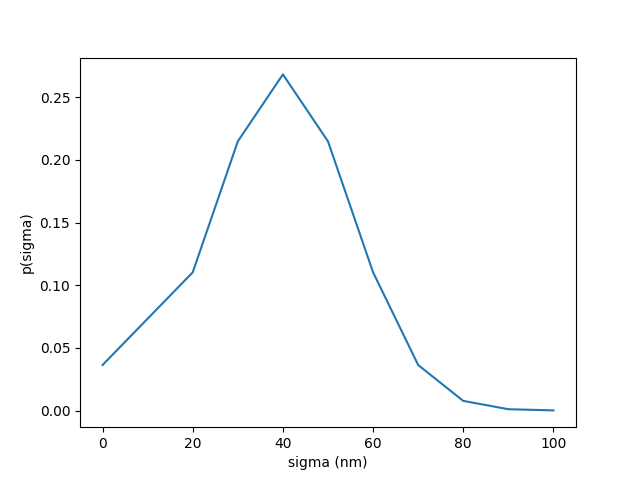
\includegraphics[width=0.5\textwidth]{figs/priorDistSigma.png}
%	\caption{}
%	\label{sigmaCurve}
%\end{figure}

\subsection{The Limitations of this model}

%The essence of this posterior probability is that is assesses how well a proposed set of clusters conforms to the expectations of the model: that each cluster has the shape of a Gaussian, and with some prior understanding of the set of labels we hope to produce\footnote{See equation \ref{priorProbability}.}


One key limitation of this model is the assumption that the clusters take the shape of a Gaussian. This is a key component of the mathematics: the fact that we assume the localisations are within a Gaussian-ring of the true molecule centres, \textit{and} that the molecule centres are within a Gaussian-ring of the cluster centres, we can use linearity to combine these "errors" into one Gaussian distribution and evaluate the necessary integrals using well-established numerical techniques. This method could be adapted to take a different probability distribution that describes the shape of non-Gaussian cell clusters, but it's unlikely that such a distribution would have a known cumulative distribution function: without this, the leap taken to arrive at equation \ref{pvGivenSigma} would be highly nontrivial, and the result would look entirely different. The authors are aware of this, and state in \cite{griffie2016bayesian} that any model is likely to have shortcomings, and whilst a Gaussian pattern provides a good fit for a wide range of situations, it's unlikely to be useful in identifying structures that are elongated or non-convex. This is not strictly true, as the results of the procedure are only a pair of values, for $R$ and $T$. The later reconstruction of the clusters in the data is agnostic to the desired characteristics of the cluster. So long as some member of a cluster has a neighbour that is within a distance of 2$R$, said neighbour will be brought into the cluster. An example of this can be seen in figure \ref{1unredclusters}(b) (particularly in the bottom left), with some large, elongated clusters clearly visible. \\



\begin{figure}
\centering
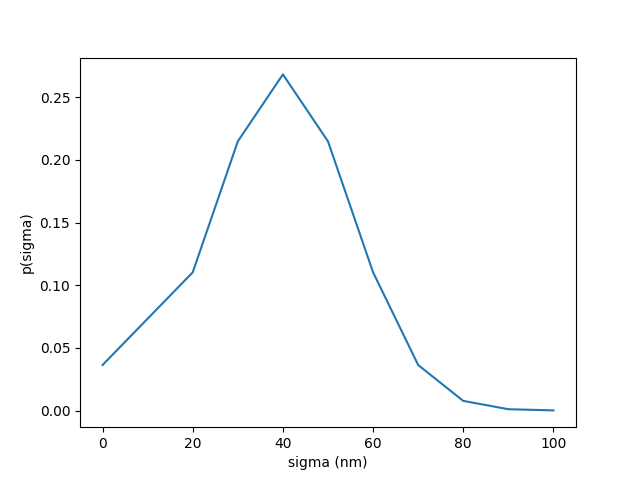
\includegraphics[width=0.4\textwidth]{figs/priorDistSigma.png}
\caption{Probability distribution for the cluster radius, $\sigma$. This is prior must be constructed with some understanding of the process being imaged. This curve was constructed with the aim of identifying clusters in an ovarian cancer cell line, tagged with an antibody against h3k9ac.
Here, this curve has a peak at 40nm, making this the favoured radius in the posterior probability calculation. See references \cite{ricci2015chromatin,xu2018super} for details on expected cluster widths in nucleosomes and h3k9ac.}
\label{fig:my_label}
\end{figure}


% \begin{figure}[t!]
% 	\centering
% 	\subfloat[\centering \textbf{caption goes here} ]{{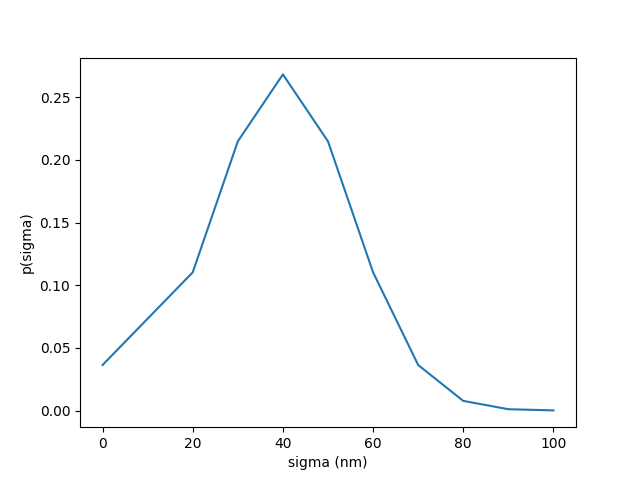
\includegraphics[width=0.4\textwidth]{figs/priorDistSigma.png} }}
% 	\qquad
% 	\subfloat[\centering \textbf{caption goes here}. ]{{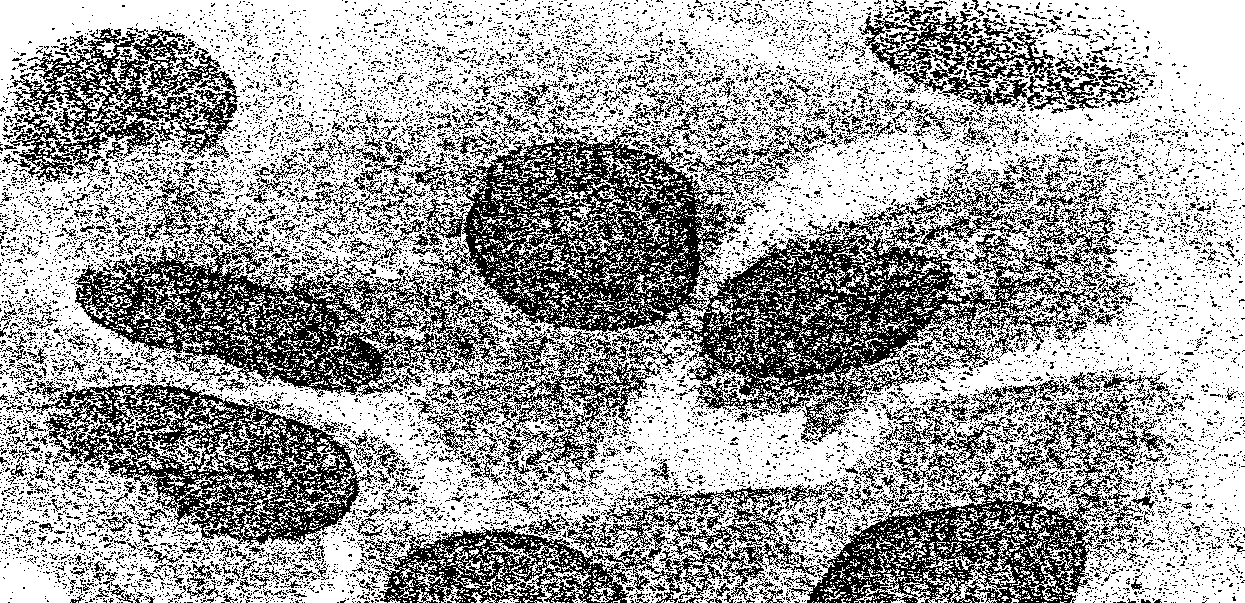
\includegraphics[width=0.4\textwidth]{figs/NP_wide_field.png} }}
% 	\caption{}%
% 	\label{SigmaCurves}
% \end{figure}

\section{Analysis of the complexity of the described algorithm}


Having outlined the algorithm in Section \ref{bayesianClusteringAlgorithm}, we turn our discussion to its practical implementation. A number of elements of the above calculation can be simplified to allow for computation that is efficient with respect to memory and other resources. In Appendix \ref{appendix:integral}, we shall rewrite the integrals above in terms of parameters which, as we shall demonstrate below allow a much more efficient use of resources when computing over a large dataset.\\


\subsection{The Algorithm, as outlined in the paper}
% \textbf{todo:}
% \begin{itemize}
% 	\item find an actual template for the algorithm to be presented in a figure
% 	\item discuss the data collection and read-in at some point before this
% 	\item ensure localisation precision are discussed in the ThunderSTORM part 
% 	\item does the above mention the two sources of the uncertainty term??
% 	\item mention the instabilities and differences between methods
% 	\item mention known limitation - we don't have high enough res to see where the actual maximum might be
% 	\item we calculate all of the localisation scores at same time as read-in
% \end{itemize}


In this subsection, we state the algorithm as outlined in the paper, before discussing in subsequent chapters how it can be made more efficient, as well as outlining its practical implementation in the current codebase.\\

The first step is to read the ThunderSTORM data in. As discussed above, the data come with three important characteristics for each molecule localisation $V_i$ - a resolved central point $(x_i, y_i)$ and a localisation uncertainty, all in nanometers. Each localisation is given a localisation score, as discussed in section \ref{localisationScore}, which is fixed for each point for the rest of the calculation, as it is a function of the number of points in immediate vicinity. Our aim at this stage is to determine which values of the clusterisation radius $R$ and the localisation threshold $T$ are the most reasonable given the data at hand. The authors scan each of these parameters from 0 to 200nm\footnote{This upper range is chosen as conventional microscopy is suitable beyond 200nm.}, and from 0 to 500 respectively, meaning that for each value of $R$ and $T$ in these specified ranges, clusters are drawn, and then scores are calculated. More specifically, the threshold $T$ is first set to some value in the range (0, 500)\footnote{Talk about skipping the early parts of the threshold}. Each datum with a score below this value of $T$ is determined to be part of the background at this stage, and is ignored until the next two values of $R$ and $T$ are determined. Each remaining datum is thus determined to be a member of a cluster of size 1 (i.e. containing just itself as a member.) The data are then scanned once more: any two localisations which are within a distance $2R$ of each other are brought together, as members of the same cluster. At this stage, we can calculate the probability that this set of labels\footnote{Labels here meaning, membership or non-membership of some cluster for each datum.} would have been issued, given the set of localisations that were observed, using the expression given in equation \ref{probLGivenV}. 


\section{The Algorithm as implemented, accounting for speedups.} \label{algImplementation}

% \textbf{todo}:
% \begin{itemize}
% 	\item describe non-repetition of log score calculation
% 	\item add a nice diagram for the clusterisation section
% 	\item we could even skip T values that are less than r since these are going to be part of the background anyway
% 	\item also mention polynomial edge correction for the localisation score calculation
% 	\item mention that we zoom in on just the cell nuclei to produce a bespoke R,T score for each region -- we can also look into scanning across the nuclei or the whole image in little windows
% 	\item mention that everything was done on lo
% \end{itemize}

The algorithm described above has been implemented in C++, primarily by Dr Andrew Rose, for the purpose of utilising all the most important features of this language, such as multithreading, high-speed memory read and write\footnote{Due to its contiguous memory allocation} and the ability to perform large parts of the computational work at compile-time, rather than at run-time. Careful uses of the features of this language, alongside some important algorithmic adaptations, mean that this implementation of the algorithm can process large amounts of data efficiently.  \\


The bulk of the computational work comes from performing the numerical integration described in section \ref{themodelitself}, but great improvements in efficiency can be found in careful variation of the $R$ and $T$ parameters. \\

\subsection{Calculation of the Integrals}

In section \ref{themodelitself}, we outlined the method that the authors of \cite{Rubin-Delanchy2015} presented for evaluation of the posterior probabilities for a set of proposed clusters. In their methodology, the process should go as follows:
\begin{itemize}
	\item Fix a pair of values ($R$,$T$)
	\item Assign each point to either the background, or to one of $m$ different clusters
	\item Once the cluster members are fixed, go through each cluster, calculating the two parameters $\bar{n}$ and $S^2$ from equations \ref{nbar} and \ref{s2}.
\end{itemize}

There are ways to substantially reduce the runtime of this section however. In appendix \ref{appendix:integral} we see that the above integral can be rewritten in terms of four variables to track which, crucially, allow us to calculate the mean weighted centre etc. whilst the localisations are being brought into the cluster, rather than having to re-read the list of localisation coordinates \textit{after} the cluster has already been drawn.\\

Comparing the implementations of the two methods (one as outlined in the paper, the other making use of speed-ups when tracking variables) revealed a slight discrepancy (by a small factor) in the value of the integrand just before performing the integral with respect to sigma, but this was small enough to have negligible effect on the posterior probabilities themselves.

\subsubsection{Cluster Formation} \label{Clusterisation}
We turn our discussion first to the way in which clusters are constructed. Starting with a set of non-background points, we group together all the points which are within a distance $2R$ of each other. The na{\"i}ve method for doing this involves passing through the set of points once, and, for each point in the set, checking which of the others are within a distance $2R$. This requires quadratically many operations before ensuring that the minimum number of clusters are returned\footnote{i.e. that we don't create a new cluster every time we observe two points within this distance of each other.}. This also doesn't take into account the fact that the cluster size might grow as we continue.\\

To eliminate much of the parallel work, we begin by transforming the representation of the data. The output of ThunderSTORM, as mentioned early, comes in the form of $x$ and $y$ coordinates within the field of view (FOV). Upon read-in we instead transform them into polar coordinates with respect to one corner of the FOV\footnote{are we sure it isn't the centre?}, before sorting each of the data-points by radial distance from the origin. This has a few benefits. First, it reduces the amount of redundant works that needs to be done, since a datum's distance from the origin can be used to infer its distance from another datum (or rather, can be used to avoid doing unnecessary work when they are certainly too far apart). Second, it allows for parallelisation. Since the data are sorted by radial distance, points which are closer to each other can be handled by separate threads. Finally, the polar coordinates can again be used to reduce the number of computations needed by using each datum's angle with respect to the corner of the FOV: two data with sufficiently large angles with respect to the $x$ axis would not be able to be neighbours, as demonstrated in figure \ref{dphi}.\\

One unexpected place in which a noticeable speed-up could be found was in the edge correction of 
localisation score calculation from equation \ref{edgecorrection}. A Taylor-expansion of this expression in $\arccos(e_i/r)$ leads to, at first order:

\begin{equation*}
	\bigg(1 + \arccos(e_1/r)/2\pi\bigg)^4
\end{equation*}

\begin{figure}
\centering
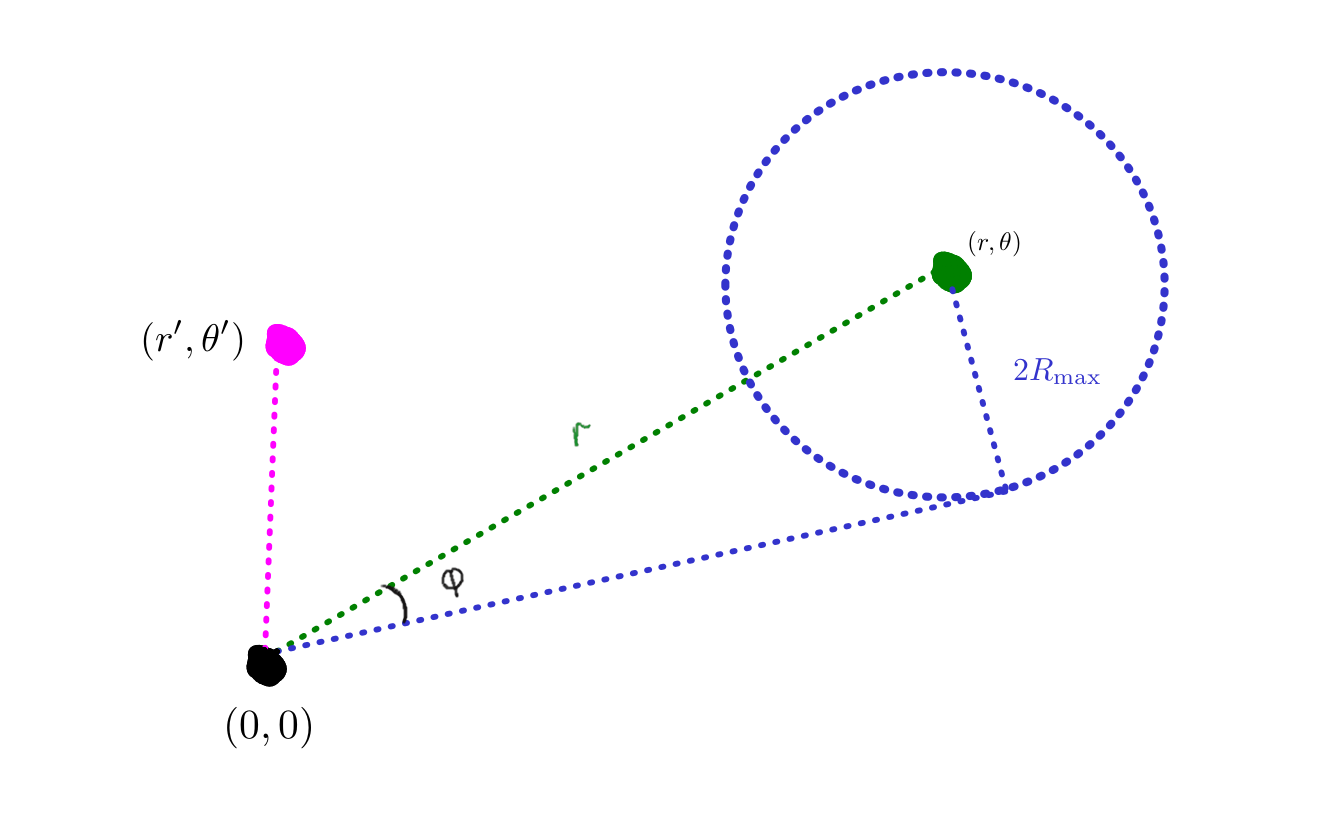
\includegraphics[width=0.5\textwidth]{figs/dphi.png}
\caption{Demonstration of an important speed-up when populating the list of neighbours of a given localisation. When searching for neighbours of the localisation located at the black dot, with polar coordinates ($r,\theta$), we first calculate $\phi$ as the inverse sin of $r / (2R_{max})$. We can then safely say that any other point with polar angle $\theta'$ will only be a candidate for the neighbour of the point at $(r,\theta)$ if $\theta - \phi < \theta' < \theta + \phi$, otherwise such a point would not be within a distance 2$R$ of the point in question. In particular, this condition on $\theta'$ determines whether or not some other localisation could be within the blue circle of radius $2R_{max}$, which is the uppermost distance any other localisation could be from $(r,\theta)$ to constitute a nearest-neighbour.  }
\label{dphi}
\end{figure}

\subsubsection{The scan over R and T}
\label{RTScan}


We can now discuss in more detail how we can determine and evaluate the clusters visible in the data whilst performing minimal redundant work during the clusterisation process. Ultimately, we require a two-dimensional scan - a value for $p(L | \nu)$ must be determined for each $(R,T)$ pair in our range of values for these parameters. \\

First, we fix $R$. We scan \textit{forwards} through the domain of $R$, meaning that on each iteration, we increase $R$ by some fixed amount (i.e. we send $R \rightarrow R + dR$). For this value of $R$, we fix a value of the threshold $T$, starting at its upper limit and working backwards towards the lower limit. The reason for computing in this order (rather than fixing $T$ at each step and then scanning through $R$) is that it doesn't require the re-drawing of the clusters. When we send $T$ to $T - dT$, data that were previously determined to be members of the background (due to their localisation score being too low), can be simply added to existing clusters, should there be some cluster that contains a datum within a distance $2R$. Moreover, if reducing the threshold doesn't add any new points to an existing cluster, we need not recalculate its integral with respect to the cluster parameters $\mu_k, \sigma_k$.





\subsection{Parallelism}

Much of the implementation exploits parallel processing, and as we shall see in section \ref{amdahlLlimit}, as we increase the number of threads available to the program we find that the eventual runtime is bounded below by the single-threaded sections. \\

We begin by describing the main sections where we exploit concurrency. Firstly, reading in the data from ThunderSTORM is sped up massively using multi-threading. The data that was used to test and validate the first version of the software contains more than 9 million lines. Each of these must be scanned to extract the central coordinates of the fluorophore, as well as its uncertainty, before determining if such a point was in the scan area. Thereafter a \texttt{Data} object is created to contain it, which also calculates some useful additional information for each datum, such as the localisation's polar coordinates with respect to the ROI. This section was a clear candidate to be parallelised: the length of the input file is first determined, so that sections of the data can be apportioned and assigned to individual threads. At this stage, no arbitration is required between threads since the data need only be added to some other container at this time.\\

Another section is the scan across R and T. As mentioned in section \ref{RTScan}, we fix a value of $R$, and calculate all posterior probabilities as we vary $T$ from its maximum value to its minimum. Once the data have been read in and pre-processed, the software establishes how many values for $R$ need to be scanned over footnote{Most experiments in this report were conducted by varying $R$ from 5 to 200nm in 100 steps.}, and crucially the number of threads that the available CPU has to offer. Each of the portions of the range for $R$ are then apportioned and sent to each of the available threads. In section \ref{amdahlLlimit} we detail the decreases in runtime that can be achieved by doing this compared to a single-threaded approach. \\


One situation in which parallelism could not be utilised fully is in the calculation of the neighbours of each datum. As a reminder, two data are \textit{neighbours} if the distance between them is less than $2R$, a parameter which varies as the scan continues. To save time, each datum is given a list of neighbours based on the maximum value of $2R$ we expect to use, which is entered when the script is initiated. Since the only criterium is that they are sufficiently close to each other, this can be used to halve the number of calculations. Once it's established that $|V_i - V_j| \leq 2R_\text{max}$, we can add $V_i$ to the list of neighbours for $V_j$ and vice versa in one calculation. One issue with that is, as discussed in section \ref{Clusterisation}, the data are sorted with respect to distance from the centre of the scan area, before fixed-size intervals of radius from the origin are passed to separate threads. This means that, at the boundary of an interval, we may find two data which ought to be neighbours, but which are being handled by different threads. Implementing this reciprocal calculation would then require either arbitration between threads to establish which data can be added to neighbour lists, or simply passing this section on one thread. Experimentation revealed that brute-forcing was the quickest way of handling this section: we divide up the data, sorted by radius from origin to each thread. Each thread then builds the neighbour list for each localisation in its domain by looking at each other datum (making use of the speed-ups mentioned in section \ref{Clusterisation}) and adding it to the neighbour list if the right conditions are met.

\subsection{Complexity Analysis}

The time and memory requirements of this implementation of this algorithm are greatly favourable compared to previous work. Through efficient use of concurrency, and minimising the number of calls to expensive functions, large speed-ups have been produced compared to prior implementations. A region containing 600,000 points takes around 2 minutes to run on a standard 8-core CPU, which is substantially quicker than times quoted in \cite{williamson2020machine}. \\

The most intensive sections are:
\begin{itemize}
	\item Determining the list of neighbours for each datum
	\item Performing the scan across the space of allowed $R$ and $T$ values.
\end{itemize}

One key optimisation that has been utilised in the development of this code was, for each datum, determining its list of nearest-neighbours once, at the start of the runtime, and sorting this list by distance from said datum. The reason for this is twofold. Firstly, it allows for the computation of all localisation scores in the initial stages of the run. Recall that each datum needs to be assigned a localisation score $L_i(r)$, which is a function of how many neighbours this datum has within a distance $r$. In accordance with the authors of \cite{Rubin-Delanchy2015}, we test 100 $R$-values between 5nm and 200nm at evenly-spaced intervals. So, equipped with a sorted list of each datum's nearest neighbours (which are all at most 200nm away), we can quickly generate the entire list of 100\footnote{Or however many proposed values for $R$ are desirable.} localisation scores for each datum. \\

Secondly, it allows for rapid drawing of clusters. When a datum has been identified as being a member of a cluster\footnote{i.e. that its localisation score is above the threshold $T$ for a particular value of this parameter.}, adding new points to the cluster is simple; iterate through this datum's list of neighbours, adding each to the cluster, until a neighbour is encountered that is further than $2R$ away; repeat this process for all the neighbours added into the cluster in the previous step.\\

One might be worried that the process of producing the list of neighbours for each datum would entail great time and space requirements. In the worst case, it would be necessary to perform $\mathcal{O}(N)$ comparisons for each of the $N$ data that were read in from the SMLM point cloud, giving it quadratic time complexity, alongside $\mathcal{O}(N\log(N))$ time to perform the sort with respect to the centre of the ROI\footnote{As mentioned in section \ref{Clusterisation}} and quadratic storage complexity, since it's necessary to store $\mathcal{O}(N)$ neighbours for each of the $N$ data. These are massive overestimates, however. It would not be necessary to perform $\on$ comparisons for each of the $N$ data. As mentioned in section \ref{Clusterisation}, we only perform comparisons when the two data are sufficiently close to each other\footnote{If the difference between the origin-to-datum distances of our point of interest and a potential neighbour is larger than $2R$, then we know they will never be members of the same cluster directly. }, and since the list of data is sorted by distance from the origin, we can safely exit execution of the produce to populate the list of neighbours. As mentioned previously\footnote{be explicit with this part}, the conversion to polar coordinates with respect to the ROI centre allows at least 1/6$^{th}$ of the potential neighbours to be ignored, due to them being unable to be within a distance $2R$ of our point of interest due to their position with respect to the origin. It is worth noting further that the list of neighbours is going to be significantly smaller than $\on$ for each datum, due to the relative size of the ROI compared with typical maximum values of $R$. A full estimate of this algorithm's complexity is beyond the scope of this report. \\

The scan across $R$ and $T$ takes up the majority of the runtime. As mentioned in section \ref{RTScan}, we increment $R$ \textit{forwards} and decrement $T$ \textit{backwards}. This requires clusters to be re-drawn only when we increment $R$\footnote{it's because threshold very low at the end of the T run. note also that localisation scores are fixed for a value of R}. Decrementing $T$ will usually increase the size of a cluster, as each cluster member is likely to have neighbours that (a) are within the \textit{clustering distance} of $2R$ units and (b) whose localisation scores are too low to be considered to be a member of a cluster. The complexity of this section is hard to establish: decrementing $T$ could require many operations, bounded above by the sum total of all elements in the list of nearest neighbours for each element already in the cluster. The likely complexity is much lower. \\

One of the most intensive sections is the calculations of various numerical integrals: fortunately the persistent state of a cluster during a scan means that these posterior probabilities are only re-calculated when the number of elements in a cluster changes, either when new points come above threshold, or when clusters accumulate due to their proximity. The real implementation of these sections relies on calls to non-standard libraries, used for interpolation and integration, the precision of which is increased with increasing resolution on the prior radius, $\sigma$. The estimation of the time required to perform these calculations is again beyond the scope of this report\footnote{\cite{williamson2020machine} gives a little more detail on the complexity considerations.}.

\subsection{Deliverables}

The main output of this procedure is an $(R,T)$ pair that most accurately encapsulates the clustering behaviour seen in the data. Following \cite{Rubin-Delanchy2015}, we present also some heatmaps, which indicate in which regions of the parameter-space one can find the highest-scoring values. One such heatmap can be seen in figure \ref{heatmap}.

\begin{figure}
\centering
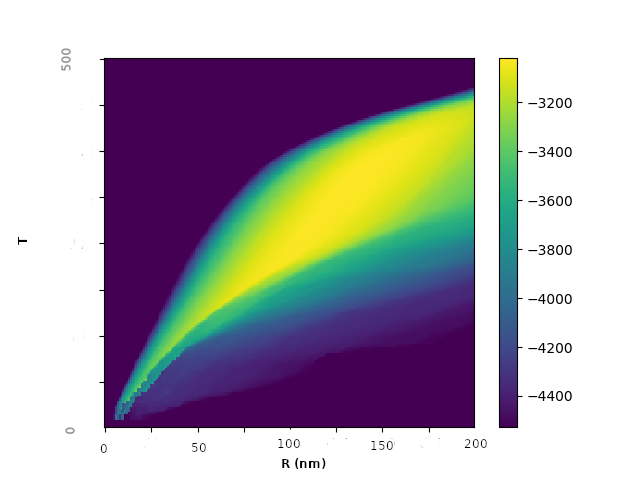
\includegraphics[width=0.7\textwidth]{figs/heatmap.png}
\caption{Heat map indicating the posterior probabilities for various $R,T$ values that were ascertained during a scan over a nucleosome dataset, which can be seen in figure \ref{standardregion}. The highest scoring pairs are indicated by the light green regions. The key for the scores, shown on the right hand side are log-probabilities, hence their large, negative values. For visual clarity, ($R,T$) pairs with scores below -4500 have been clipped to -4500. An image of the raw data, with identified clusters highlighted, can be seen in figure \ref{1unredclusters}.}
\label{heatmap}
\end{figure}
 



\subsection{Contributions and Validation}

As mentioned above, much of the codebase was already implemented before beginning this project by Dr Andrew Rose, namely the algorithmic speed-ups identified in this chapter, the inclusion of the use of multithreading, and the structuring of the code to primarily use lightweight wrappers for data, rather than having to process large amounts of raw data at every computational step. The contributions of this report were as follows.
Firstly, the validation of the mathematics within, particularly with regard to confirming that the alternative formulation of the two numerical integrals was indeed equivalent to the process outlined in \cite{Rubin-Delanchy2015}.
Secondly, the validation of the function of the code. At the beginning of this project, the majority of the posterior probabilities calculated by the code were being calculated to be \texttt{inf} or \texttt{NaN}, indicating that at some process in the pipeline was causing erroneous zero-division, or taking \texttt{log} of zero, or other such errors. After careful debugging and analysis of the flow of the code, it was determined that the main source of the \texttt{NaN} scores was the enormous difference in scale that arises when performing Bayesian calculations \cite{Rubin-Delanchy2015}. Much of the calculation in the code is performed on the log scale, per the suggestion of the authors, meaning that when the time comes to perform mathematical operations such as those in equation \ref{sigmaintegral}, values must be exponentiated before doing so. Unfortunately, doing so would often require exponentiated a number at least as large as $10^2$, which is too large for the precision of the C++ type \texttt{double}. At stages like this, a scaling factor is introduced so that values to be exponentiated are reduced to be $\leq 0 $, preventing infinite numbers effectively "poisoning" later calculation, with scaling factors being later removed when appropriate.
Other contributions to this project include a robust method to identify regions of interest, as described in section \ref{timings}, as well as the validation of the clustering behaviour and the inclusion of a method to determine the most optimal $R,T$ pair at runtime.





\section{Experimentation}


In this chapter, we present our results from the computational experiments performed using the high-performance tool described above. 

\subsection{Timings}
\label{timings}
Our aim was to process a 96-well plate in six colour channels in under 24 hours. We present evidence here that using a supercomputing cluster will certainly facilitate this. Figure \ref{standardregion} shows a scan of some nucleosomes, which have been labelled with a fluorophore. In particular, what we see is an ovarian cancer cell line, tagged with an antibody against the histone h3k9ac, and a secondary antibody conjugated with Alexa 647.  Clearly visible are at least 8 nuclei. One na{\"i}ve way of performing this is to simply scan over the whole region at once, but there are a number of issues with this. Primarily, the idea of of performing this kind of scan is to produce a pair of parameters that will identify clusters within a given ROI, on a meaningful scale. A reasonable pair of values might be three orders of magnitude smaller than the width of the ROI. Moreover, the characteristics of each cell might be vastly different between nuclei, and perhaps within nuclei as well. Moreover, as we discussed in the section on complexity\footnote{do so concretely}, processing possible tens of millions of data-points at once would be prohibitively costly in memory and time.\\

The first approach was to simply cut down the ROI. A separate scan would be run over each nucleus. The nucleus can be identified manually, but for the sake of running automated scans, we outline a tool that can be used to do so automatically. A coarse scan of the image is taken as a two-dimensional vector, before performing a Gaussian blur. The effect of this can be seen in figure \ref{blurprocess}. This causes regions of higher pixel-density (and hence with more localisations) to be brightened and less dense regions to be darkened. After setting a minimum pixel brightness threshold, the identified nuclei can be seen. From there comes a simple breadth-first search\footnote{include this as an algorithm} to determine the ROIs necessary to scan over each of the nuclei. \\

We outline here the results of scanning across the various nuclei shown in figures\footnote{put these figures in}. The localisations within these regions of interest were scanned, one at a time, on a single 64-core CPU. Cumulatively, these regions contain over 8 million points, with individual nuclei containing between 680,000 and 2.3 million localisations. The total time taken for all of the processes to run sequentially was less than 25 minutes. \\

Further to this, we demonstrate the runtime of a variety of different scans, each performed over the same nucleus with the same central focus, but with progressively wider regions of interest and hence progressively more points encapsulated in the scans, in figure \ref{1unredclusters}. 

\begin{figure}
\centering
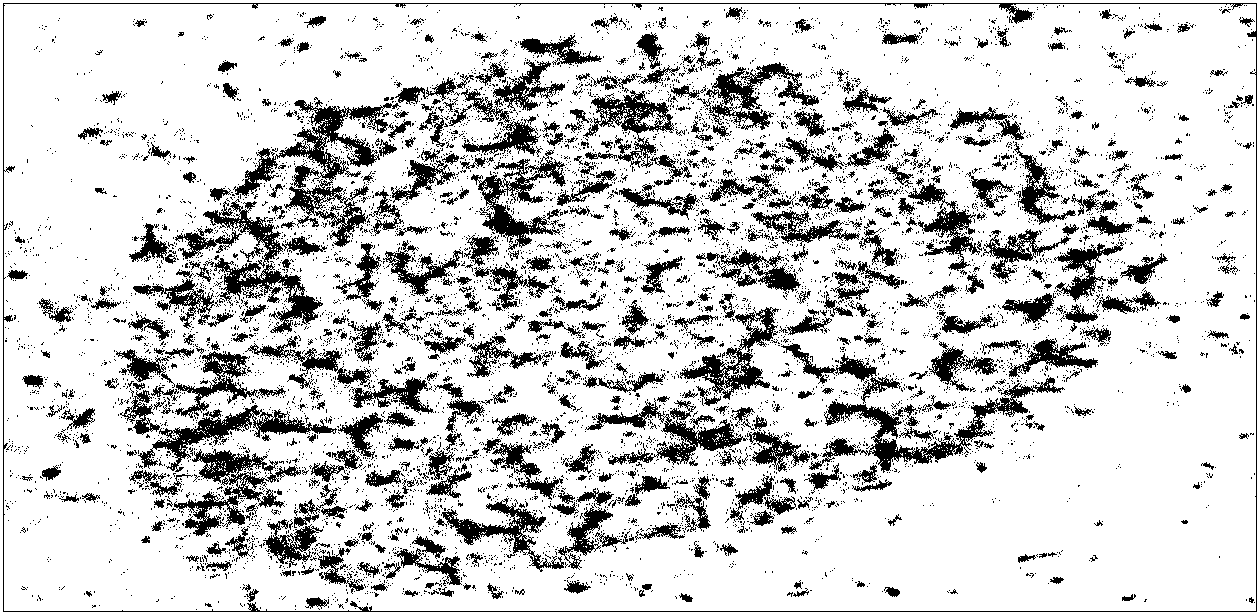
\includegraphics[width=0.7\textwidth]{figs/87_32_standard_region.png}
\caption{Representative image of an SMLM dataset, which has been tagged with the fluorophore Alexa 647 to produce localisations.}
\label{standardregion}
\end{figure}

\begin{figure}[h!]
	\centering
	\subfloat[\centering Low resolution scan of an SMLM dataset, also seen in figure \ref{standardregion}. ]{\raisebox{5ex}{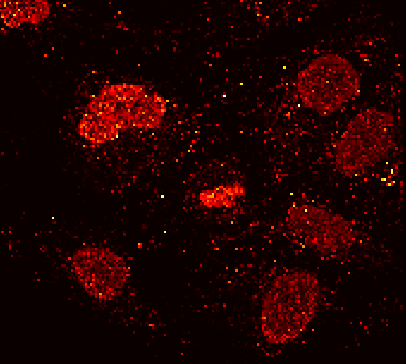
\includegraphics[width=0.3\textwidth]{Beamerposter—flow multicolumn/figs/1_un_red_csv_raw.png}
	}}
	\qquad
	\subfloat[\centering The same image as part (a), having undergone a Gaussian blur. ]{{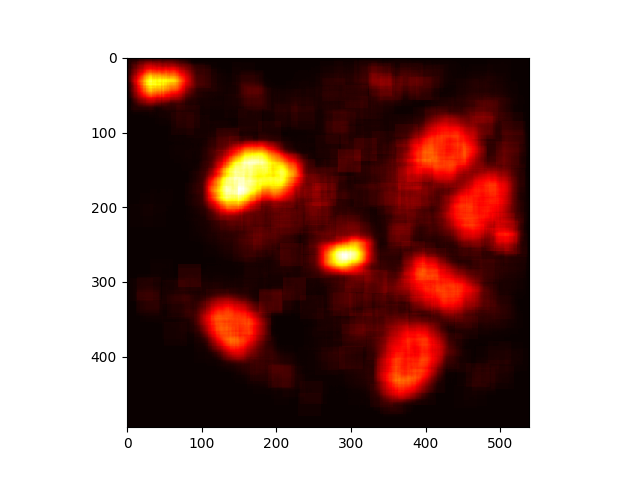
\includegraphics[width=0.5\textwidth]{Beamerposter—flow multicolumn/figs/blur.png} }}
% 	\subfloat[\centering \textbf{caption goes here}. ]{{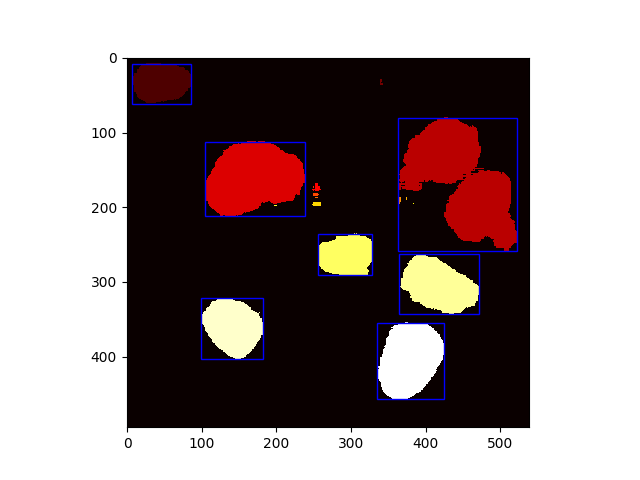
\includegraphics[width=0.5\textwidth]{Beamerposter—flow multicolumn/figs/clustered.png} }}
	\caption{These two figure show the first two steps in the identification of nuclei to perform scans over. After these two steps, the pixels whose brightness values are too low will be set to 0.}%
	\label{blurprocess}
\end{figure}

\begin{figure}[h!]
    \centering
    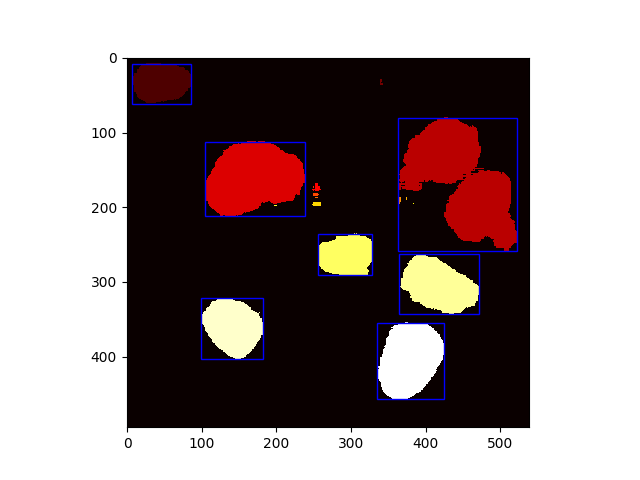
\includegraphics[width=0.5\textwidth]{Beamerposter—flow multicolumn/figs/clustered.png}
    \caption{Caption}
    \label{After the pixel values in figure \ref{blurprocess} have been thresholded, the \textit{islands} within the image can be identified, and constitute the regions of interest to perform a scan over. }
\end{figure}


\subsection{Memory Usage} \label{chapter:memusage}

We present here a short demonstration that the peak memory usage of the procedure is linear with respect to the number of localisations being analysed at once. Figure \ref{memusage} shows a scan of a nucleus\footnote{which kind}. The clustering procedure was run on square ROIs, with widths varying from 1$\mu$m to 25$\mu$m, capturing between 2500 and 930,000 localisations. \ref{memusage}(b) demonstrates a clear linear relationship between the peak memory usage and number of points. Processing 930,000 points had a peak memory usage of 63.8GB, which may be important for future sizing of jobs.

\begin{figure}[t!]
	\centering
	\subfloat[\centering \textbf{Maximum memory usage of the procedure in megabytes, against number of points included in the ROI. } molecule.]{{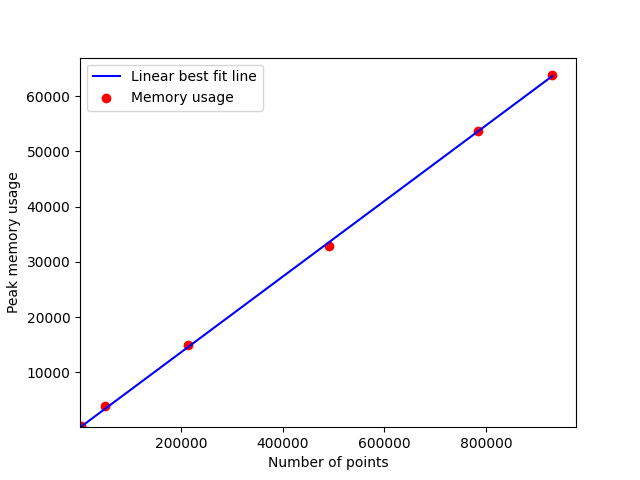
\includegraphics[width=0.7\textwidth]{figs/memusage.png} }}
	\qquad
	\subfloat[\centering \textbf{The region the scan was performed over.} ]{{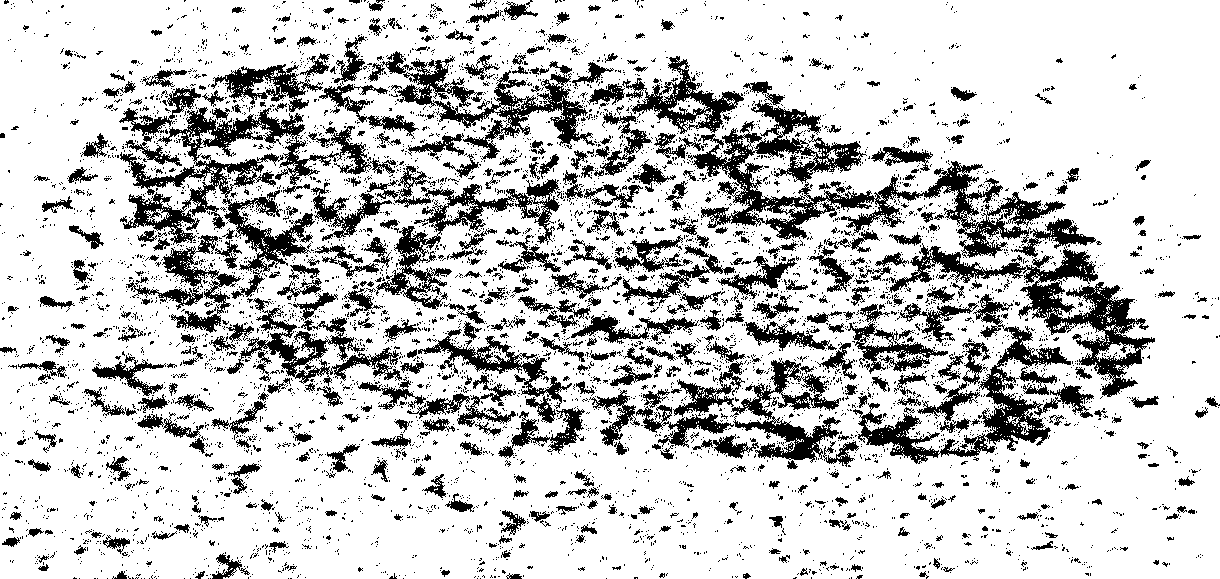
\includegraphics[width=0.6\textwidth]{figs/memusage_97_90.png} }}
	\caption{The graph in part (a) shows the peak memory usage in megabytes of the procedure, for 5 differently-sized regions of interest, each with the same central point, but with varying ROI width. The graph shows a clear linear relationship between peak memory usage and number of points analysed.}%
	\label{memusage}
\end{figure}

\subsection{ROI Sizing}

%Here we show the comparison between scanning nuclei individually, compared with moving a small window across the entire ROI. We do this both to compare the values of $R$ and $T$ gained therefrom, but also to compare the running times in both scenarios.
The results from section \ref{chapter:memusage}, also demonstrated that the parameters $R$ and $T$ returned by the procedure can vary somewhat substantially when altering the region of interest. In particular, as we included more points into a larger ROI, with both values for $R$ and $T$ rising until plateau, before a slight fall as the entire nucleus was brought into the field-of-view. An interesting question to answer for a future work is whether the nature of clusters in biological systems is highly specific to individual regions within nuclei, or whether clusters formed are characteristic of a more macro-process, such as the regions between and around cells. When scanning each of the visible nuclei in section \ref{timings}, each produced a different $R$-value, but a fairly consistent $T$-value. We present figures for each in the\footnote{appendix}.


\begin{figure}[t!]
	\centering
	\subfloat[\centering Diagram of the nucleus seen in figure \ref{standardregion}, with the identified clusters for $R$=46nm, and $T$ = 114. The width of the ROI is 15$\mu$m ]{{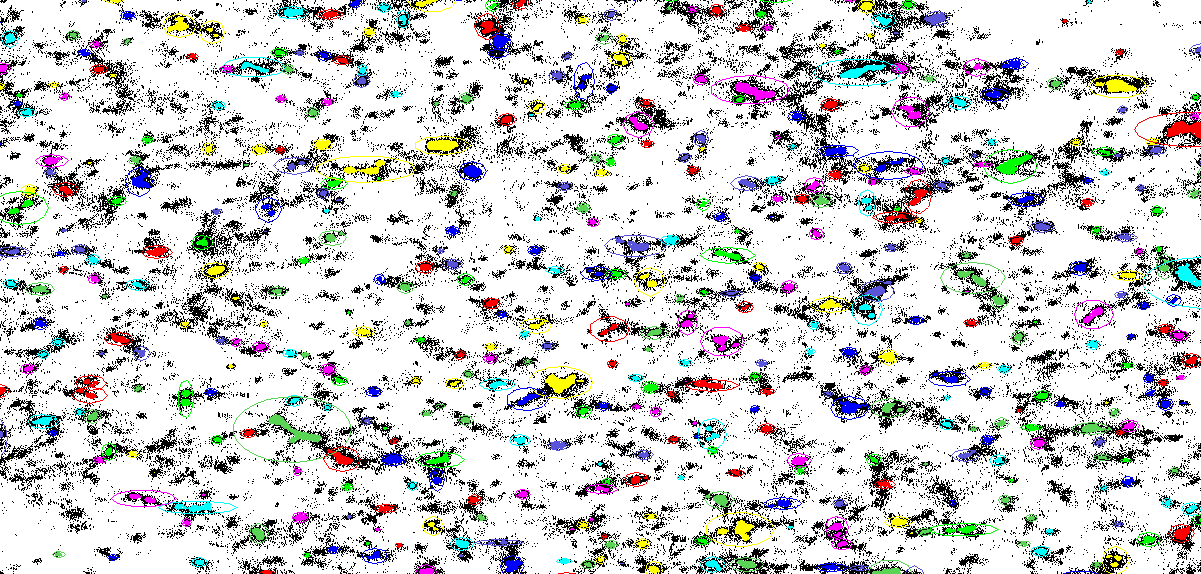
\includegraphics[width=0.8\textwidth]{figs/46_114_wide.png} }}
	\qquad
	\subfloat[\centering The same as figure (a), but with a ROI width of 5$\mu$m. ]{{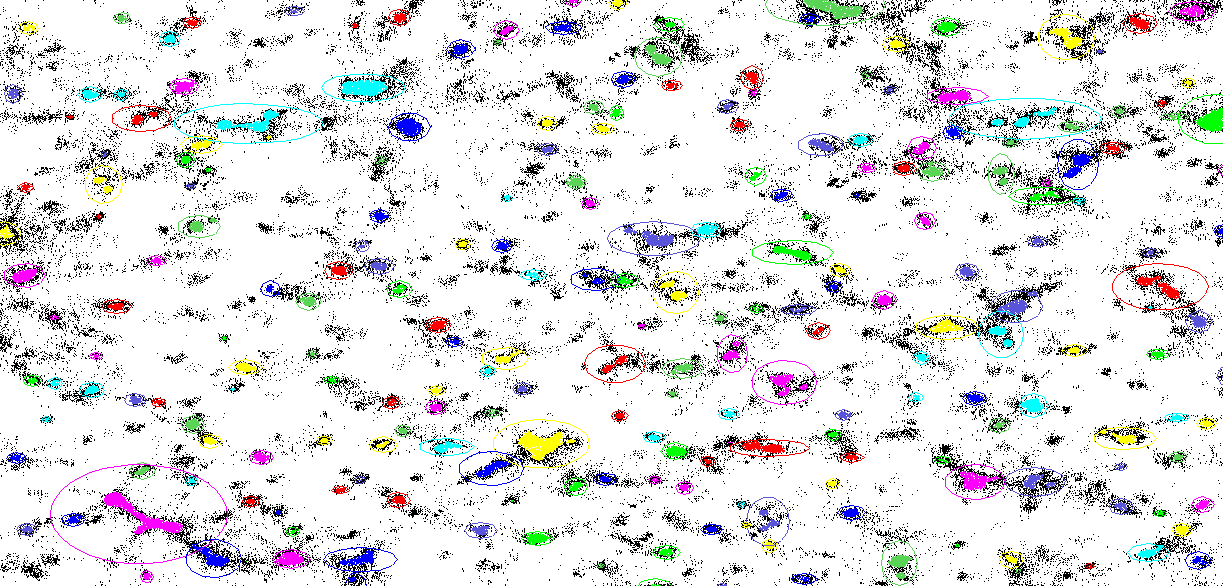
\includegraphics[width=0.8\textwidth]{figs/46_114_narrow.png} }}
	\caption{}%
	\label{1unredclusters}
\end{figure}


%
% \begin{figure}
%     \centering
% 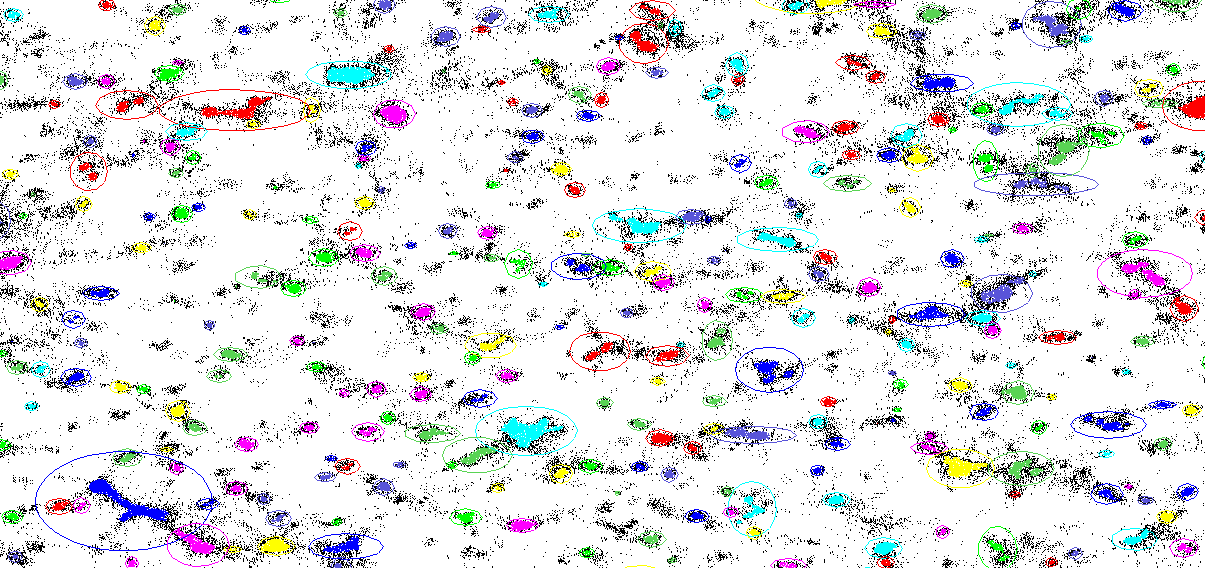
\includegraphics[width=0.8\textwidth]{figs/32_74.png}
%     \caption{The same region as seen in figure \ref{1unredclusters}(b), but with $R,T$ = 32nm,74. This pair of values was determined by the algorithm to be the most optimal when analysing the 5}
%     \label{1unredclusters2}
% \end{figure}



\subsection{Nuclear Pore Testing}




In this section we describe using this cluster-identification process on a well-understood dataset which can serve as a ground truth. Given that we know many of the essential characteristics of this dataset, such as expected number of localisations per cluster and expected cluster radius, we can use this to evaluate the performance of this algorithm\footnote{move this sentence}. We can also, using the clusters we identify, measure the error incurred during the imaging process, by comparing the width of the cluster identified in the image to their known width. \\


%\section{ground truthing}
%\subsection{nucleopore dataset}
%\textbf{see paper in comment its local and also sent by miqi}
%/home/seanbaccas/Documents/maths/MSC/MScProject/maybeClustering/groundTruth/Nuclear_Pore_Jonas_Ries.pdf
\subsubsection{Nuclear Pores as a reference standard}
\label{npReferenceStandard}

One persistent issue in the study of imaging biological systems is their seeming lack of reproducibility. Many aspects need to be taken into account when analysing samples, such as the precise settings of the optics equipment and the fluorophores used in labelling. Thevathasan et al. \cite{Thevathasan2019} are aware of this, and discuss which commonly-imaged cell structures can provide some kind of "ground-truth" when imaging cells with SMLM. They make the case for the nuclear pore complex (NPC) as an ideal reference structure, as it has consistent characteristics that allow for extraneous parameters to be optimised, given the knowledge of what to expect within the region of interest itself. In particular, the NPC contains roughly 30 different proteins, for which a high resolution electron-microscope map already exists.  \\

Figure \ref{npDiag} (reproduced from \cite{Thevathasan2019}) shows some of the characteristics we can expect from nuclear pore complexes, namely rings of proteins with consistent diameters. This allows us to tailor our prior probability curve for sigma, as described in section \ref{sigmacurvediscussion}\footnote{inculde the sigma curve here}. Figure \ref{npDiags} shows a scan from some SMLM-acquired images in both the wide-field of 40$\mu$m by 40$\mu$m, as well as a much closer scan of 5$\mu$m by 5$\mu$m. Highlighted with red boxes are some locations of the nuclear pore rings described above. The images taken from them are not precise - the rings themselves contain too many localisations, as well as their overall pattern has been blurred away from a neat octagon. There are many possible explanations for this. Firstly, the imaging technique at hand takes places stochastically over several minutes, meaning that fluorophores may drift away from their positions at some time between their first emission and the end of the final imaging cycle. This means that a fluorophore that blinks multiple times in different positions cannot be easily filtered from the data, as it may appear as more than one distinct localisation. Secondly, these images were taken from 3D structures, and whilst TIRF\footnote{make sure this is explained} microscopy aims to draw an image from a flat plane, this doesn't always prevent some photon emissions from depth being found in the final localisation table. \\

In the following section we will detail how this implementation of the algorithm performed in the identification of clusters on NPC data.


\begin{figure}
\centering
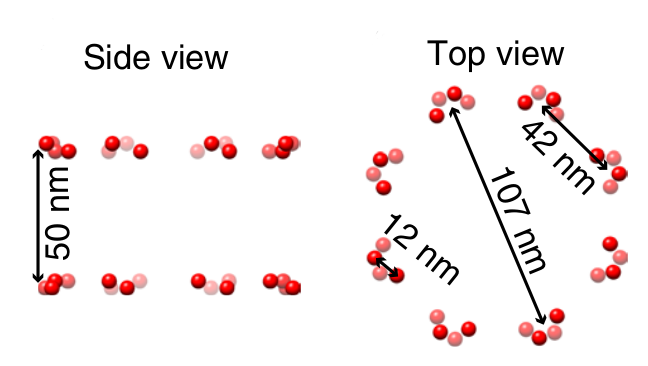
\includegraphics[width=0.5\textwidth]{figs/np.png}
\caption{Part of figure 1 from \cite{Thevathasan2019}. The nuclear pore complex (NPC) has predictable characteristics - we typically find groups of the protein Nup96 forming octagonal rings, with two octagons stacked atop each other. These rings have predictable characteristics: the corners consist of a proteins with a width of 12nm; the side length of this octagonal shape is consistently 42nm, with diameter of 107nm.}
\label{npDiag}
\end{figure}


\begin{figure}[t!]
	\centering
	\subfloat[\centering Scan of a nuclear pore dataset, ROI width 80$\mu$m. ]{{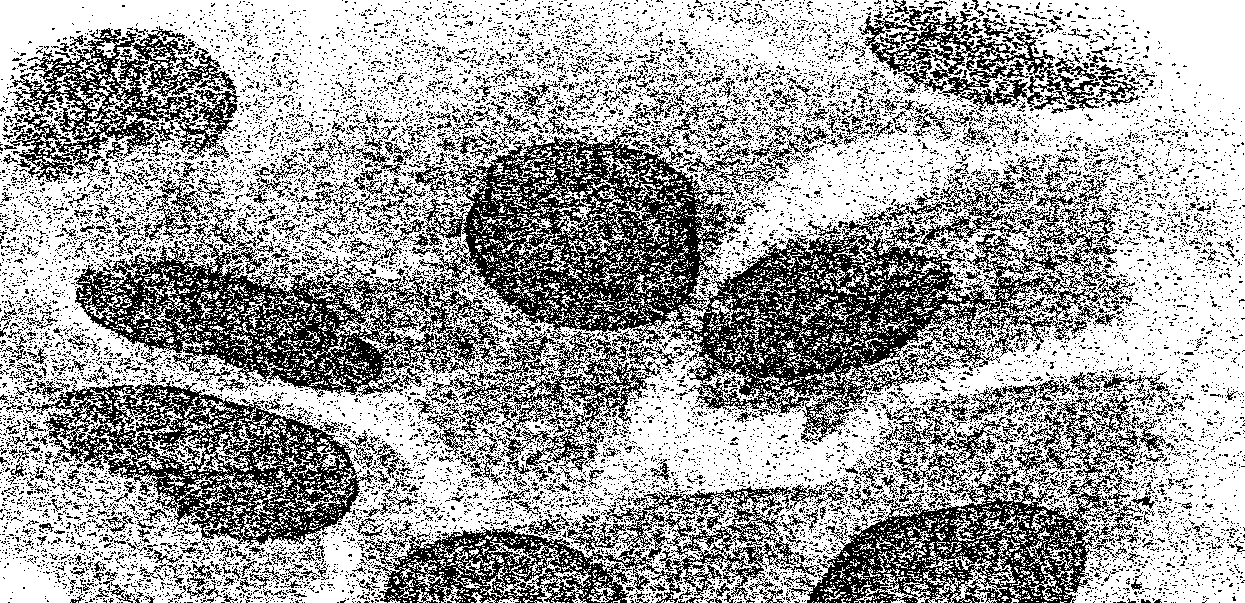
\includegraphics[width=0.4\textwidth]{figs/NP_wide_field.png} }}
	\qquad
	\subfloat[\centering Closer scan of the same image, with ROI width approximately 5$\mu$m. Highlighted in red are the relevant protein clusters which we aim to seek out with the cluster identification procedure. ]{{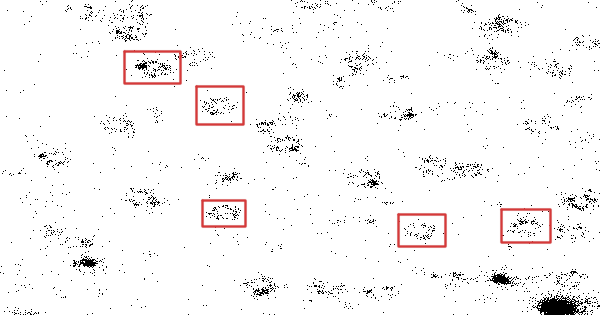
\includegraphics[width=0.4\textwidth]{figs/1_NP.png} }}
	\caption{This figure shows a scan of a nuclear pore complex. Zooming in closely reveals the predictable pattern of the protein clusters.}%
	\label{npDiags}
\end{figure}


%we have no way to optimise the configs of all the factors we need to be correct such as hardware setup and analysis software. So we turn to "suitable reference standards". simulated images served as reference standards to benchmark software - see [8] within. we can create artificial reference structures. The so-called nuclear pore complex satisifies a lot of things we need for a good artificial dataset. we even have an electron microscopy thing to use. they demonstrate why they are useful, they use it for (1) quantify microscope performance,
%resolution and calibration, (2) measure absolute labeling efficien-
%cies, (3) optimize imaging conditions and (4) count protein num-
%bers within a complex. \textbf{resolution and quality control} Apparently SMLM shows clear rings and strarts resolving the \textbf{eight} corners. the effective labelling efficinies section suggests that some cell line they have produces few blinks - ie they won't show up in some frame more than once. \\
%
%SMLM allows counting of proteins in dense structure, but relating the number of localisations to the number of proteins is tricky. we can get undercounting and overcounting. \textbf{we need faithful segmentation}. 

\subsubsection{The experiments themselves}

For this part of the experimentation, we used a localisation table which was gathered from a nuclear pore sample. Figure \ref{npDiags}(a) shows an image taken from the localisation table. The field of view is approximately 80$\mu m$ by 80$\mu m$. Clearly identifiable are at least 8 nuclei, surrounded by a lot of noise, most of which can be attributed to the cytoplasm background. We see here that, in spite of TIRF microscopy being able to image a fairly "flat" plane in 3d space, we see here a lot of localisations from other depths. As we zoom closer in to a section of the image, as shown in \ref{1_NP}, we can begin to identify the nuclear pores themselves. In these images, the distinctive \textbf{8-localisation} structure is tricky to identify. Rather than forming an octagon, most of the pores we can see have been blurred into a ring, or loop. \\

There are a number of possible explanations for this. The SMLM process itself can introduce errors. Over the few minutes of imaging time, molecules are prone to drifting, and later releasing another photon during a subsequent imaging round. In combination with this, the process through which localisations are generated (by detecting the parameters of a Gaussian within the pixelated point spread function) can introduce further errors. Some simple filtering methods were not effective: ThunderSTORM localisation tables come with a "sigma" parameter, which describes the width of the observed PSF. We expect Alexa-647 to produce PSFs of width 160-200nm\cite{thunderstorm}. Filtering for this still produced noisy, inconsistent data.\\

The blur of the imaging process can be seen in figure \ref{1_NP}. We have a close-up image of a likely nuclear pore. The centre still has an identifiable "gap", forming the shape of a ring. We have far higher localisations here than expected. Even when taking into account the number of localisations per cluster we see in our ground truth data\footnote{as mentioned beforehand}, we have approximately ten times more localisations here than expected from a nuclear pore. Some of these will be background points, as nuclear pores are three-dimensional structures, which perhaps highlights the limits of precision available with conventional microscopy.\\

Performing cluster analysis was much less straightforward on this dataset compared to histone data, such as was discussed in section \ref{timings}. To summarise the method used there, we began by using a Gaussian blur to identify the dense regions (the visible nuclei) before reducing the ROI to enclose only one nucleus and running the scan to produce an optimal $R$ and $T$ value for this nucleus. In the case of the nuclear pore data available, scanning over a region much larger than 25 square $\mu m$ caused the posterior probabilities\footnote{Posterior probabilities indicate which $(R,T)$ pair is optimal.} to indicate highly unrealistic values for $R$ and $T$. As a result, the scans were performed with a \textit{sliding window} of 4$\mu m$ by 4$\mu m$ with the hope of finding an optimal pair of values that can identify clusters over the whole dataset. An important fail-safe when evaluating clusters is to ascertain that areas which are clearly clustered together are identified by the algorithm: eye-balling is often a good place to start if otherwise unsure. \\

Picking an appropriate probability density curve for cluster radius, sigma was slightly tricky also. As discussed previously, prior study of nuclear pore complexes has revealed a few distinct, predictable substructures visible in the images. Figure \ref{SigmaCurves}(b) illustrates this: we aim to prioritise the larger clusters of width 107nm, as well as the smaller clusters of width 12nm. The curve for the first round of scans can be seen in figure \ref{onePeakSigma}. Some results were initially promising, with multiple nuclear pore clusters being identified in the FOV. However, the results of the algorithm appeared too heavily biased towards large threshold values. This meant that whilst the values for $R$ led often to sensible clusters being identified in some regions, many others were missed. This was due to the $T$ parameter being too high: any other potential clusters were simply labelled as background points\footnote{Include some figures to illustrate what is meant}. \\

To counter this, multiple new scans were done, but instead strictly limiting the scan values for $R$ and $T$, after observing the cluster behaviour when manually modifying the parameters. I found that threshold $T$ being too high was the main issue. Finding a pair of values that produces a few clusters\footnote{see figures} was not too difficult, however these values would cause the cluster-drawing to avoid many of the clusters which appeared to be obvious to the naked eye. As can be seen in figure\footnote{add said figure}, increasing the value of $R$ beyond realistic values simply causes multiple pseudo-clusters to be brought together, whereas in figure\footnote{add this fig}, increasing the threshold allows more clusters to be identified.\\

Rather than the classic scan ranges, of 0 to 200nm for $R$ and 0 to 500 for $T$, the ranges for subsequent scans were restricted to 20 to 150nm for $R$ and 0 to 200nm for $T$. In spite of using a curve which is perhaps non optimal, one particularly good pair of values was $R=$28nm and $T=141$. Figure\footnote{include it} shows the identified clusters at a range of ROI widths. We can see at this values, a good proportion of the clusters have been located, but we search still for more optimal values. \ref{ThreePeakSigma}\\
%inside 6111567

These results were built on by adjusting the sigma curve to the one found in figure \ref{ThreePeakSigma}. The idea behind using this, modified curve was to encourage the algorithm to \textit{reward} identifying clusters with those particular radii.\\

The dataset used was quite tricky to analyse. Correctly tagging nuclear pores with Alexa 647 is time-consuming, and can is prone to failure\footnote{check this}. Moreover, localisation density within nuclear pores is not uniform, suggesting that this method is not suitable here. Clustering, in this model, is determined by comparison with CSR\footnote{Or in other words, uniform randomness} which may not be possible if rate of change of localisation density with respect to any of the coordinates is too large. This may also preclude the use of a small sliding window to determine optimal $(R,T)$ parameters: how does one generalise the use of a pair of values to any region outside where it was determined.
Beyond the scope of this report is a discussion on whether better data may be gathered for such an analysis, and whether the algorithm can be adapted to be more suitable for this scenario, perhaps by introducing some pressure towards a certain number of localisations per cluster\footnote{mention this in the outro - also mention that they found the sigma curve doesn't really matter, so this hampered efforts to makes sure it was good}. Possible avenues of investigation for a future work include using the width clusters identified by the Bayesian procedure (whose width can be measured computationally) to provide some estimate of the errors that occurred during the imaging and localisation process.  \\

% \begin{figure} 
	
% 	\centering
% 	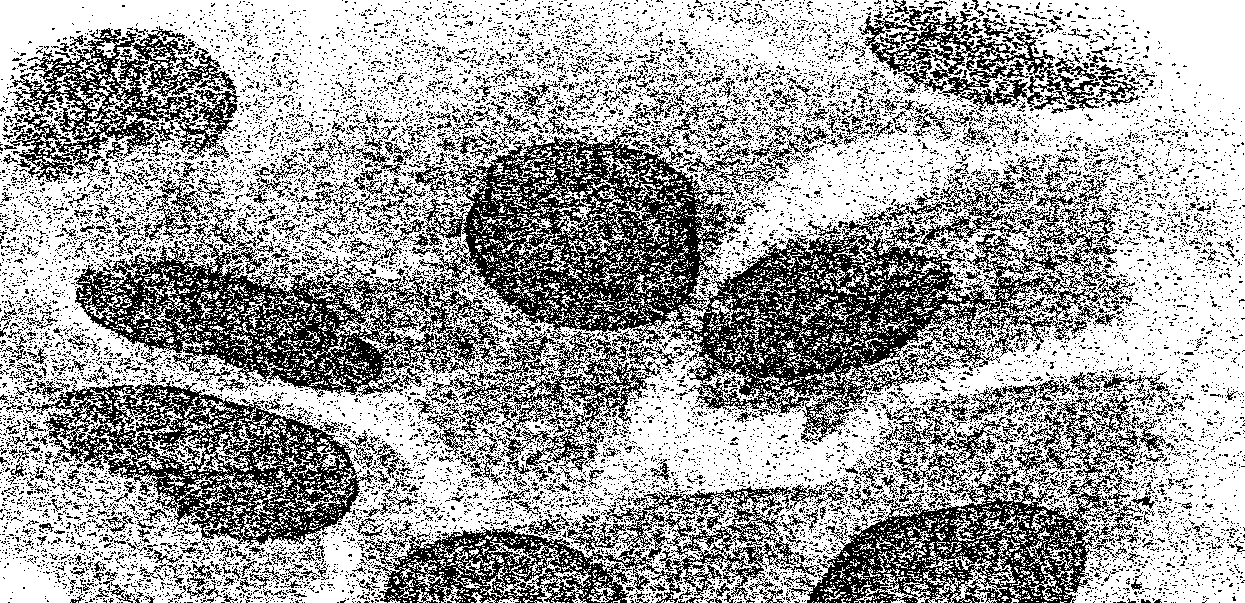
\includegraphics[width=0.9\textwidth]{figs/NP_wide_field.png}	
% 	\caption{Scan of a nuclear pore complex image}
% 	\label{NP_wide_field}
% \end{figure}
%\begin{figure} 
%	
%	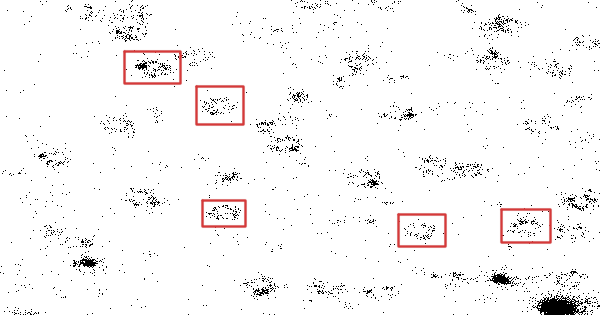
\includegraphics[width=0.9\textwidth]{figs/1_NP.png}
%	\caption{\textbf{include a slightly more zoomed out one, not nec the same thing}}
%	\label{1_NP}
%\end{figure}



\begin{figure}[t!]
	\centering
	\subfloat[\centering Wide field scan of a nuclear pore complex, with ROI width 15$\mu$m. ]{{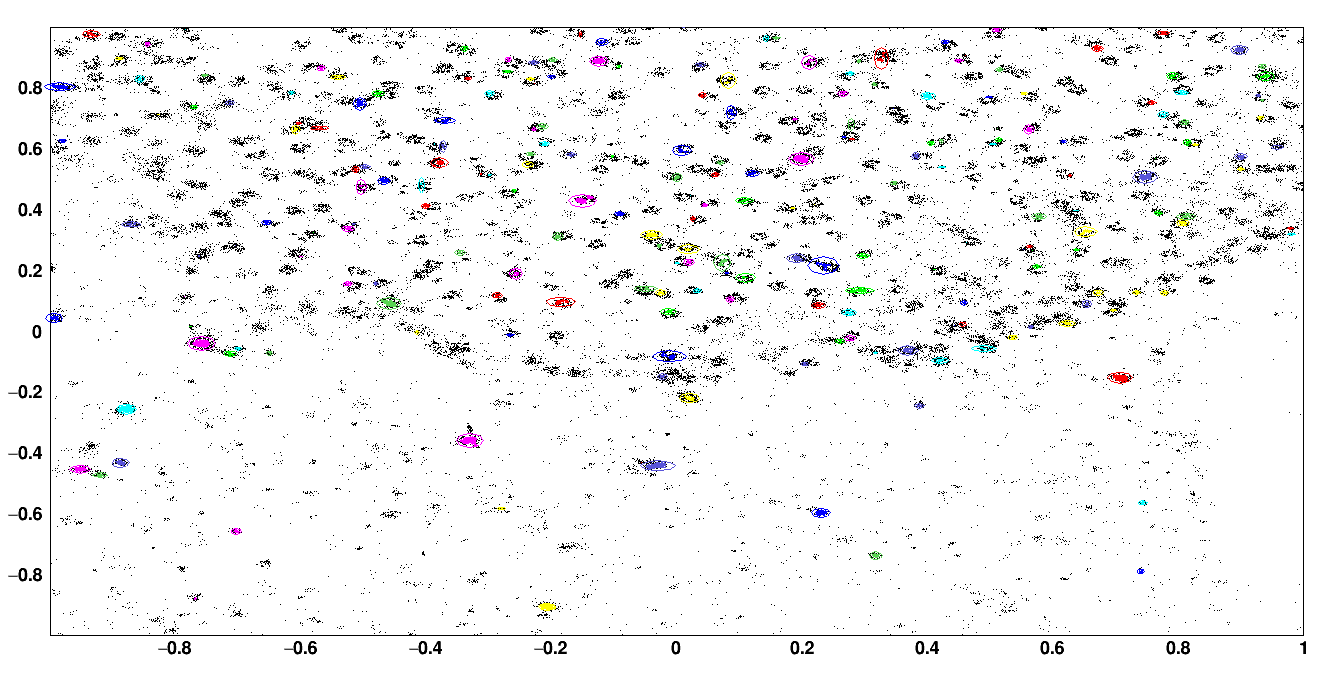
\includegraphics[width=0.9\textwidth]{figs/NP_26_117_wide.png} }}
	\qquad
	\subfloat[\centering Narrow field scan of a nuclear pore complex, with ROI width 5$\mu$m. ]{{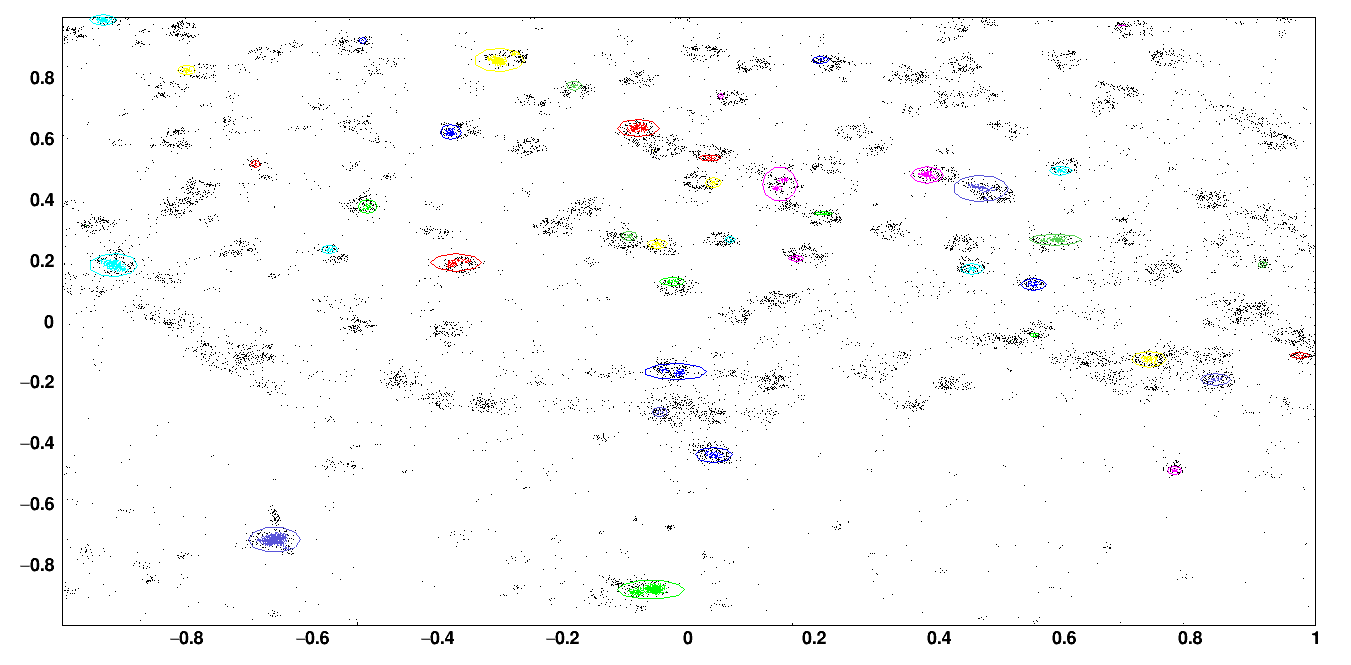
\includegraphics[width=0.9\textwidth]{figs/NP_26_117_narrow.png} }}
	\caption{Two scans of the nuclear pore complex from figure \ref{npDiags}. The procedure determined the values $R,T$ = 26nm, 117 to be the most optimal. Not all of the clusters were identified, even when looking at the wide field image.  }%
	\label{npClusters}
\end{figure}


%\begin{figure} 
%	\label{NP_wide_field}
%	\centering
%	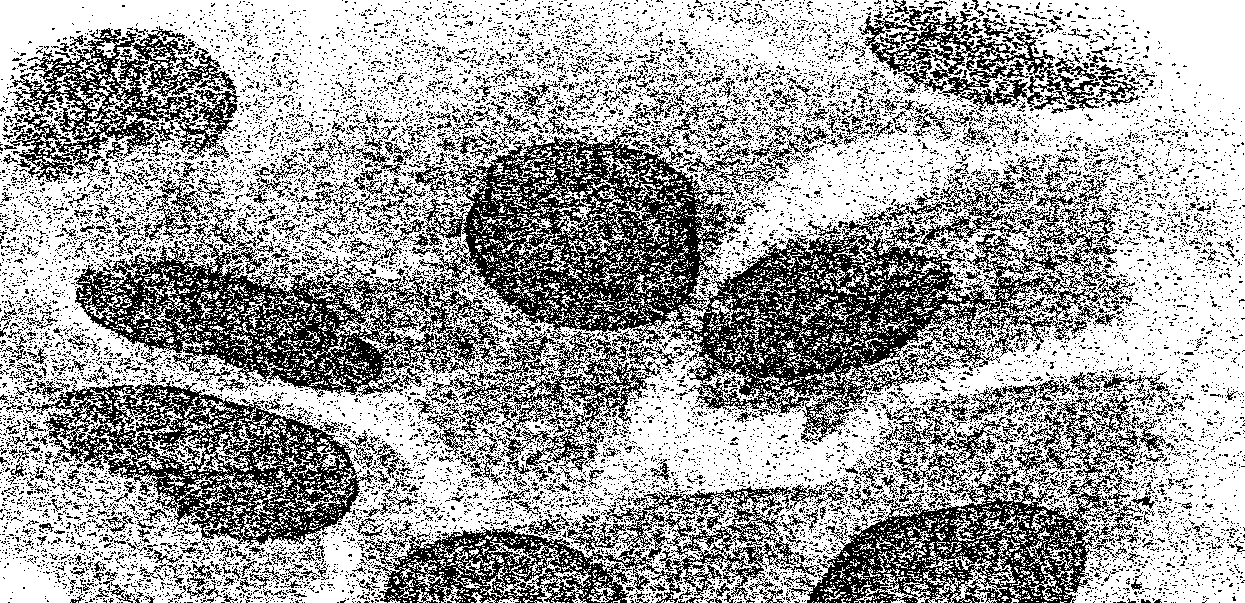
\includegraphics[width=0.9\textwidth]{figs/NP_wide_field.png}	
%	\caption{Caption}
%\end{figure}
%\begin{figure} 
%	\label{1_NP}
%	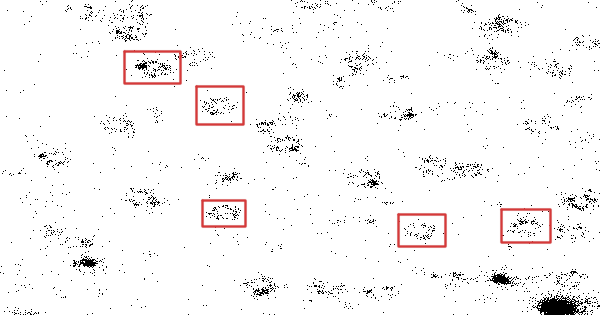
\includegraphics[width=0.9\textwidth]{figs/1_NP.png}
%	\caption{\textbf{include a slightly more zoomed out one, not nec the same thing}}
%\end{figure}
%\begin{figure} 
%	\label{onePeakSigma}
%	\centering
%	\includegraphics[width=0.5\textwidth]{figs/OneDipSigma.png}
%	\caption{\textbf{include a slightly more zoomed out one, not nec the same thing}}
%\end{figure}
%\begin{figure} 
%	\label{ThreePeakSigma}
%	\centering
%	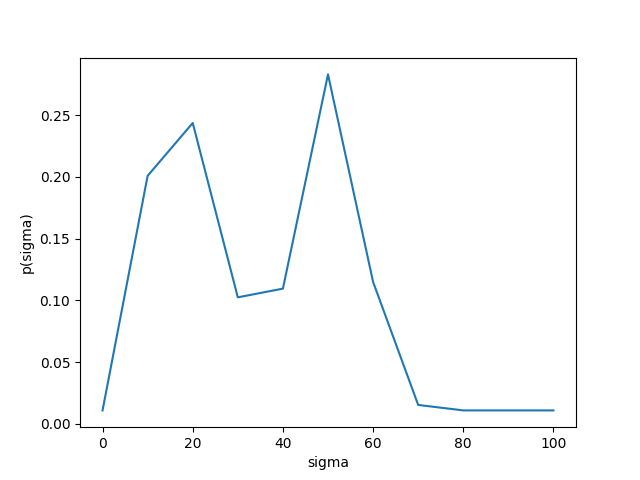
\includegraphics[width=0.5\textwidth]{figs/threeDipSigma.png}
%	\caption{\textbf{include a slightly more zoomed out one, not nec the same thing}}
%\end{figure}

\subsubsection{Synthetic Data}

A much more clear view of the performance of this model can be seen when looking at synthetically-produced data, carrying on from the work of \cite{williamson2020machine}. Their idea was to analyse the performance of clustering algorithms against a clean dataset with known priors. We present here the results of scanning over 9 datasets, each of which have a few (varying) parameters with which we can assess the performance of the Bayesian method. These parameters include:
\begin{itemize}
	\item The number of points in the FOV
	\item The number of points in each cluster
	\item The proportion of points that belong to the background
	\item The number of clusters in the ROI
	\item The maximum cluster radius
\end{itemize}

The results are summarised in table \ref{syntheticTable}. The efficiency and purity of this method are both high. Each of the datasets contained over 40,000 points, each of which had a target for the percentage of points belonging to clusters set at either 25\% or 50\%. In every case, the algorithm made an incorrect decision for less than 1\% of the members of the simulated dataset. The number of identified clusters was highly accurate too, the error on which was typically less than 5\%. For instance, when analysing the seventh dataset, the values we expected to find were as follows\footnote{change the list: irrelevant info therein}:
\begin{itemize}
	\item Number of points per cluster: 20
	\item Maximum Radius per cluster: 40nm
	\item Percentage of points assigned to clusters: 25\%
\end{itemize}

Out of 46064 points viewed by the algorithm, a correct class label (cluster or background) was given in 45917 places, a success rate of more than 99\%. Of the ones that were labelled incorrectly, 81 background points, and 66 cluster members, were given the opposite class label. It's worth noting that the model assumes the background points are uniformly distributed across the FOV: given that we have approximately 0.2\% of the FOV covered by clusters, we may expect that of the approximately 35,000 background points in the dataset, around 70 of them should still appear within an identified cluster. We were able to detect 569 clusters, compared to the target of 584. This is likely attributable to clusters in close proximity being drawn together - this is behaviour that can occur due to the choice of the $R$ parameter.. \\

We believe that this demonstrates the algorithm is capable of performing highly accurate clustering on SMLM data. What remains to be seen is how this algorithm copes with a more varied dataset, synthetic or otherwise. One interesting thing to note from \cite{williamson2020machine} is Figure 3(g), which shows the Bayesian method is inaccurate when analysing a CSR background. One suggestion may be to, below a certain posterior probability\footnote{A low posterior probability would indicate that }, add some pressure to the algorithm to raise the threshold $T$, to ensure that points are not erroneously clustered together.\\




\begin{figure}
\centering
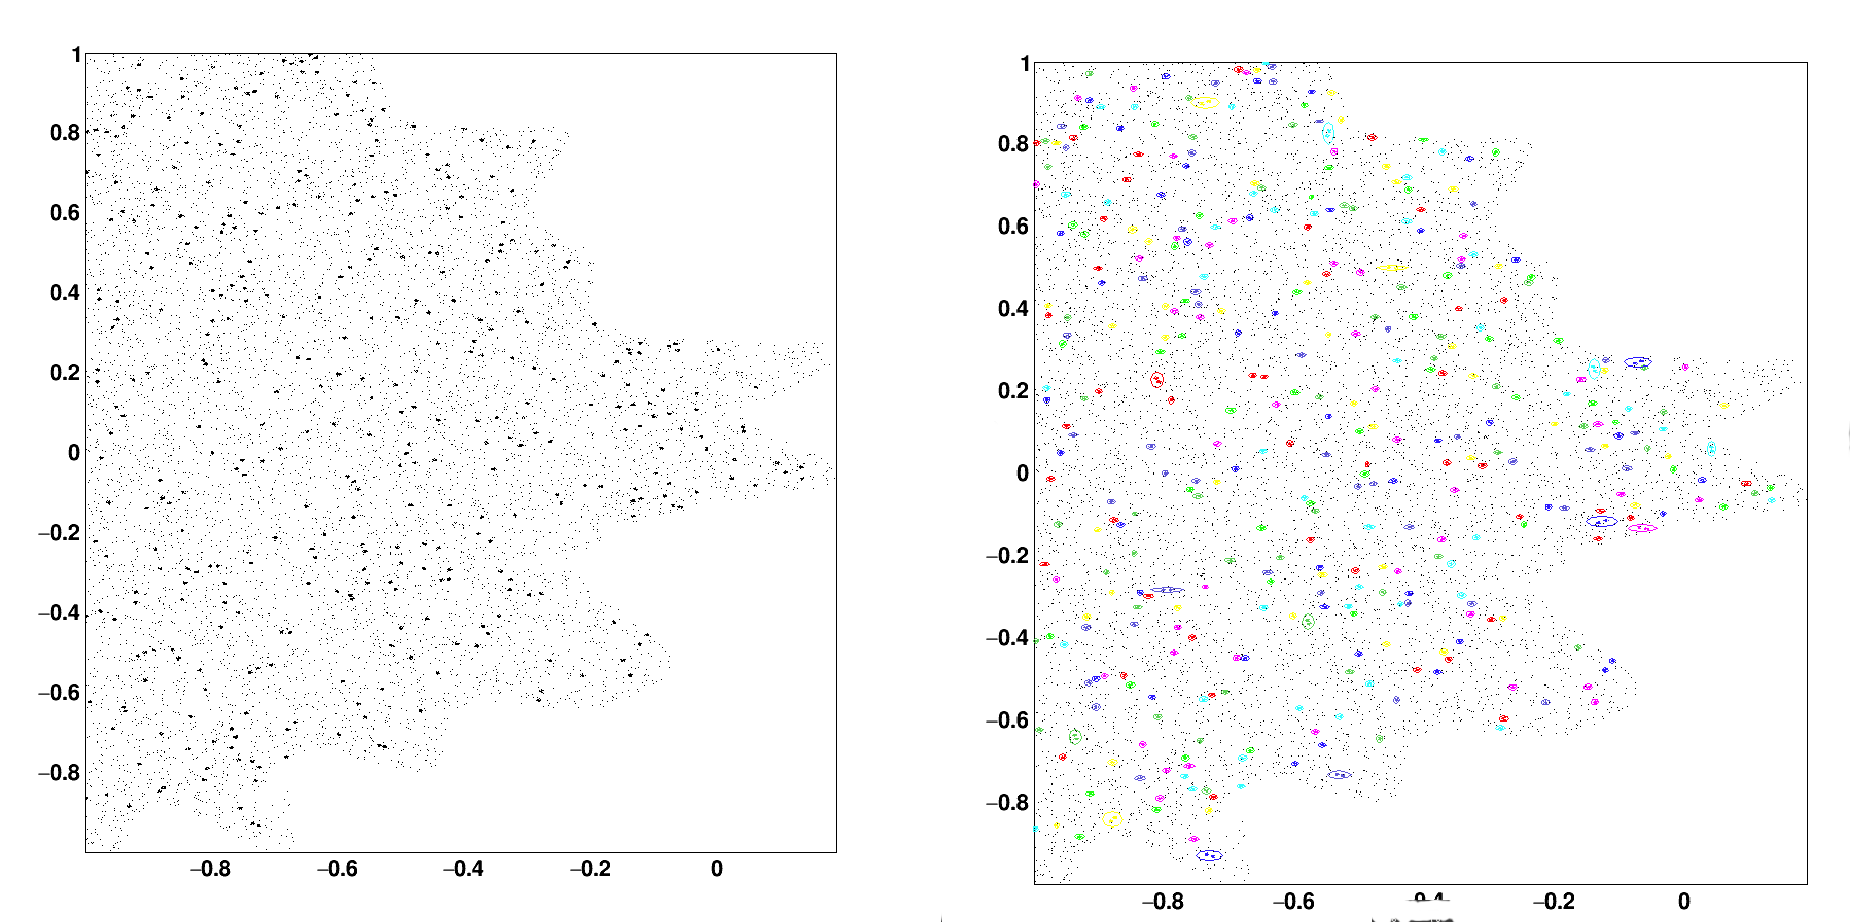
\includegraphics[width=0.99\textwidth]{figs/syntheticFig.png}
\caption{Representative scan of a procedurally generated dataset, based on the work of \cite{williamson2020machine}. On the left we see the raw data, and on the right the identified clusters are overlaid.}
\label{syntheticFig}
\end{figure}

% \subsubsection{Sensitivity to parameters}
% \label{RTsensitivity}
% Rubin-Delanchy et al. \cite{williamson2020machine} have discussed the robustness of this algorithm with respect to various parameters. The main contribution of this report is empirical evidence that their procedure can be implemented in a way that allows for high-throughput analysis of SMLM data, and so in the following section we demonstrate how the diagrams of the identified clusters change with respect to the parameters $R$ and $T$.

\subsection{Limits of Multithreading}
\label{amdahlLlimit}

We present here a brief demonstration that the use of multithreading allows us to maximise the possible gains in runtime. We ran 7 different scans of the nucleus seen in figure \ref{standardregion}, the first using a single thread, before each time doubling the number of threads in use to a maximum of 64. Figure \ref{standardregion} shows the results. We see that initial increases in thread counts lead to extremely rapid decreases in runtime: the process of both populating the neighbour lists and scanning across the $R-T$ parameter space halved each time the thread count was increased from 1 to 2, then from 2 to 4 and finally from 4 to 8. Thereafter, the decreases in runtime plateau, as we reach some kind of bottleneck, as the portions of the code which cannot be multithreaded begin to dominate the runtime.
Beyond the scope of this project is a thorough investigation into what dominates the runtime of the code when fully parallelised, such as calls to non-standard libraries that interpolate functions and calculate numerical integrals.

\begin{figure}
\centering
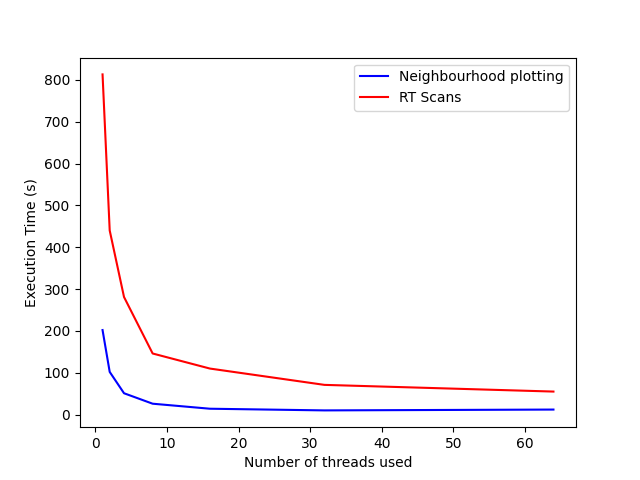
\includegraphics[width=0.7\textwidth]{figs/multithread.png}
\caption{Plot of the execution time of two parts of the procedure against number of threads used.}
\label{multithread}
\end{figure}




\section{Future Work}
\label{notyetimplemented}
We could avoid scanning R values below T - these are indistinguishable from CSR. Getis and Franklin \cite{getisAndFranklin} designed the localisation score measure to satisfy $L_i(r) = r$ for points generated by the Poisson process. Unless determining whether a pointillist dataset resembles a CSR, looking for clustering with $T \leq R$ is not necessary and these portions of the computational work can be avoided. \\

We may also wish to introduce some penalty to the posterior probability to \textit{encourage} the algorithm to fall inside some desirable bounds, such as number of localisations per cluster.
The authors of \cite{datta2006methods} introduce some measure for evaluating the analysis produced by a clustering procedure. While this may be good to give some indication of a post-hoc quality of the identified clusters, we leave it up to future work to discuss how such measures could either be used to modify the cluster identification procedure, or to modify the calculation of posterior probabilities, so that the procedure may produce more biologically-realistic clusters.
As it currently stands, it is not well understood how small changes in $R$ and $T$ can alter the nature of the identified clusters. Currently, our only way of evaluating the clustering behaviour is with respect to the model outlined in section \ref{thebayesianmodel}. 

\section*{Conclusion}

In this project we demonstrated that an efficient, high-performance implementation of a Bayesian method for evaluating clusters in SMLM data is possible. We began with a discussion on SMLM and microscopy, outlying the importance of searching for clustered regions in SMLM data. 


\newpage		
\nocite{*}
\bibliographystyle{plain} % We choose the "plain" reference style
\bibliography{litReview}


\appendix

\newpage
\section{The Integral}
\label{appendix:integral}
The following is adapted from unpublished work by Dr Andrew Rose.

In equation \ref{localisationGivenParameters}, we stated that for a given cluster containing $n$ localisations, the probability of observing this set of localisations, given cluster parameters $\mu = (\mu_x, \mu_y)$ and $\sigma$ was given as a product of probabilities. We begin our discussion with the calculation of each of these $n$ terms. We stated further that we can write this probability as:

\begin{align*}
	p(V_{i}\,|\,\mu,\sigma) \eq  \frac{1}{2\pi\sig^2}\ \text{exp}\left( \frac{-(x_{i}-\mu_x)^2 }{ 2\sig^2 }  - \frac{(y_{i}-\mu_y)^2 }{ 2\sig^2 }\right),
\end{align*}

where we have defined $\sig = \sigma^2 + s_i^2$, the sum of our two standard deviations\footnote{ensure this is properly defined somewhere}. For each cluster identified, we aim to compute the integral within. Let us now expand this integral to reveal some quantities which can allow for efficient calculation of these probability densities. Due to the separability of the gaussian, we can consider integrating over each spatial dimension of the Gaussian independently. Without loss of generality, we consider the $x$ dimension:

\begin{align} \label{muIntegralOneDimension}
	\int_{x-}^{x+} \prod_{i=1}^{N} & \left( \frac{1}{\sqrt{2\pi\sig^2}} \text{exp}\left( \frac{-(x_i-\mu)^2 }{ 2\sig^2 }\right)\right)\,d\mu \nonumber \\
	\eq \int_{x-}^{x+} \left(\prod_{i=1}^{N} \frac{1}{\sqrt{2\pi\sig^2}}\right)\left(\prod_{i=1}^{N} \text{exp}\left( \frac{-(x_i-\mu)^2 }{ 2\sig^2 }\right)\right)\,d\mu \nonumber \\
	\eq \left(\prod_{i=1}^{N} \frac{1}{\sqrt{2\pi\sig^2}}\right) \int_{x-}^{x+} \prod_{i=1}^{N} \text{exp}\left( \frac{-(x_i-\mu)^2 }{ 2\sig^2 }\right)\,d\mu \nonumber \\
	\eq \left(\prod_{i=1}^{N} \frac{1}{\sqrt{2\pi\sig^2}}\right) \int_{x-}^{x+} \text{exp}\left( -\sum_{i=1}^{N} \frac{(x_i-\mu)^2 }{ 2\sig^2 }\right)\,d\mu.
\end{align}

We next examine the sum inside the integral:

\begin{align*}
	\sum_{i=1}^{N} \frac{(x_i-\mu)^2 }{ 2\sig^2 } 
	\eq \frac{1}{2}\left( \mu^{2}\sum_{i=1}^{N}\frac{1}{\sig^2} - 2\mu\sum_{i=1}^{N}\frac{x_i}{\sig^2} + \sum_{i=1}^{N}\frac{x_i^2}{\sig^2} \right) \\
	\eq \frac{1}{2}\left( A\mu^{2} - 2B\mu + C \right) \\
	\eq \frac{1}{2}\left( A(\mu - D)^2 + E \right).                                                 
\end{align*}

Above, we have defined:

\begin{align}
	A \eq \sum_{i=1}^{N}\frac{1}{\sig^2} \\
	B_d \eq \sum_{i=1}^{N}\frac{x_{d,i}}{\sig^2} = AD_d \\
	C_d \eq \sum_{i=1}^{N}\frac{x_{d,i}^2}{\sig^2} = AD_d^2 + E_d = \frac{B_d^2}{A} + E_d \\     
	D_d \eq \frac{B_d}{A} \\
	E_d \eq C_d - AD_d^2 = C_d - \frac{B_d^2}{A}.
\end{align}

Based on our earlier discussion of the necessary calculation that needs to be performed, we can demonstrate how the above variables fit in to the general picture. Taking the integral from equation \ref{muIntegralOneDimension}, and removing the constant factor $ \frac{1}{\sqrt{2\pi\sig^2}}$, we can state that:

\begin{align*}
	\int_{x-}^{x+} \prod_{i=1}^{N} & \left(  \text{exp}\left( \frac{-(x_i-\mu)^2 }{ 2\sig^2 }\right)\right)\,d\mu \\
	\int_{x^-}^{x^+} & \text{exp}\left( -\sum_{i=1}^{N} \frac{(x_i-\mu)^2 }{ 2\sig^2 } \right)\,d\mu \nonumber \\
	\eq \int_{x^-}^{x^+} \text{exp}\left( -\frac{1}{2}\left( A(\mu - D)^2 + E \right) \right)\,d\mu \\
	\eq \int_{x^-}^{x^+} \text{exp}\left(-\frac{E}{2}\right) \text{exp}\left( -\frac{1}{2}\left( A(\mu - D)^2 \right) \right)\,d\mu \\
	\eq \text{exp}\left(-\frac{E}{2}\right) \int_{x^-}^{x^+} \text{exp}\left( -\frac{1}{2}\left( A(\mu - D)^2 \right) \right)\,d\mu \\
	\eq \text{exp}\left(-\frac{E}{2}\right) \int_{x^-}^{x^+} \text{exp}\left( \frac{-(\mu - D)^2}{2\frac{1}{A}}\right)\,d\mu \\
	\eq \text{exp}\left(-\frac{E}{2}\right) \int_{x^-}^{x^+} \frac{\sqrt{2\pi\frac{1}{A}}}{\sqrt{2\pi\frac{1}{A}}} \text{exp}\left( \frac{-(\mu - D)^2}{2\frac{1}{A}}\right)\,d\mu \\
	\eq \sqrt{\frac{2\pi}{A}}\cdot\text{exp}\left(-\frac{E}{2}\right) \int_{x^-}^{x^+} \frac{1}{\sqrt{2\pi\frac{1}{A}}} \text{exp}\left( \frac{-(\mu - D)^2}{2\frac{1}{A}}\right)\,d\mu \\
	\eq \sqrt{\frac{2\pi}{A}}\cdot\text{exp}\left(-\frac{E}{2}\right) \left[ \phi\left(\frac{x^+-D}{\sqrt{\frac{1}{A}}}\right) - \phi\left(\frac{x^--D}{\sqrt{\frac{1}{A}}}\right) \right] \\
	\eq \sqrt{\frac{2\pi}{A}}\cdot\text{exp}\left(-\frac{E}{2}\right) \left[ \phi\left(\sqrt{A}(x^+-D)\right) - \phi\left(\sqrt{A}(x^--D)\right) \right] \\
	\eq \sqrt{\frac{2\pi}{A}}\cdot\text{exp}\left(-\frac{E}{2}\right) \cdot G.
\end{align*}

Here we have defined:

\begin{align*}
	G_d \eq \phi\left(\sqrt{A}(x_d^+-D_d)\right) - \phi\left(\sqrt{A}(x_d^--D_d)\right)
\end{align*}

with:

\begin{align*}
	\Phi(x) = \int_{-\infty}^{x} (2\pi)^{-1/2} \exp(-y^2 / 2) dy
\end{align*}

being the standard Gaussian cumulative distribution function. We can then continue - the probability of observing a set of localisations $\nu = [V_1, V_2, \dots, V_N]$ requires taking the product of $p(V_i | \mu, \sigma)$ for each $V_i$ in $\nu$, before integrating over the $\mu$ and $\sigma$ parameters. 

\begin{align} \label{numericallyUnstableIntegral}
	p( \nu ) \eq \ints p(\sigma) \intm p(\mu) \prod_{i=1}^{N} p(V_{i}\,|\,\mu,\sigma)\,d\mu\,d\sigma \nonumber \\
	\eq \ints p(\sigma) \prod_d \left[ \frac{1}{(x_d^+ - x_d^-)} \left(\prod_{i=1}^{N} \frac{1}{\sqrt{2\pi\sig^2}}\right)\sqrt{\frac{2\pi}{A}}\text{exp}\left(-\frac{E_d}{2}\right)G_d \right]\,d\sigma \nonumber \\  
	\eq (2\pi)^{(1-N)\cdot\tau/2} \cdot V^{-1} \ints p(\sigma) \cdot \left(\prod_{i=1}^{N} \frac{1}{\sig^2}\right)^{\tau/2} \cdot A^{-\tau/2} \cdot \prod_d\left[\text{exp}\left(-\frac{E_d}{2}\right)\right] \cdot \prod_d G_d \,d\sigma \nonumber \\
	\eq (2\pi)^{(1-N)\cdot\tau/2} \cdot V^{-1} \ints p(\sigma) \cdot F^{\tau/2} \cdot A^{-\tau/2} \cdot \text{exp}\left(-\frac{1}{2}\sum_d E_d\right) \cdot \prod_d G_d \,d\sigma \nonumber \\
	\eq (2\pi)^{(1-N)\cdot\tau/2} \cdot V^{-1} \ints p(\sigma)\cdot\left(\frac{F}{A}\right)^{\tau/2}\cdot\text{exp}\left(-\frac{E}{2}\right) \cdot \prod_d G_d \,d\sigma 
\end{align}

Where:

\begin{align}
	E \eq \sum_d E_d 
	= \sum_d (C_d - B_d D_d) \nonumber \\
	\eq \sum_d C_d - \sum_d B_d D_d \nonumber \\
	\eq C - \sum_d B_d D_d \nonumber \\
	C \eq \sum_d C_d 
	= \sum_d \sum_{i=1}^{N} \frac{x_{d,i}^2}{\sig^2} 	\nonumber \\
	\eq \sum_{i=1}^{N} \frac{\sum_d x_{d,i}^2}{\sig^2}	
	= \sum_{i=1}^{N}\frac{r_i^2}{\sig^2}  \\
	F \eq \prod_{i=1}^{N} \frac{1}{\sig^2}  
\end{align} 


We can now choose these four variables to track, and we shall rewrite some important equations in terms of them. In later sections, we shall demonstrate how tracking these variables during the cluster proposal process allows for (at least one) fewer passes of the whole set of localisations. Per the suggestion of \cite{Rubin-Delanchy2015}, the large difference in scales means that this computation must be performed on the log scale. In particular, the scale differences can be so large that, as we shall see in later sections\footnote{REF!}, computation must be performed carefully to ensure that all variables remain within the confines of the type \texttt{double}. We find that the integrand in equation \ref{numericallyUnstableIntegral} is numerically unstable, and so calculation of these quantities is performed on the log scale, and then exponentiated just before the numerical integration step. \\

Turning our attention back to the prior probability we noted in equation \ref{priorProbability}, we state here its log-scale expression.

\begin{align*}
	ln\left(p\left(l\right)\right) \eq n_{B}\cdot ln\left(p_B\right) + (N-n_B)\cdot ln\left(1-p_B\right) + m\cdot ln\left(\alpha\right) \nonumber \\
	& + ln\left(\Gamma\left(\alpha\right)\right) + ln\left(\prod_{k=1}^{m}\Gamma\left(n_k\right)\right) - ln\left(\Gamma\left(\alpha + N - n_B\right)\right) \\
	\eq n_{B}\cdot ln\left(p_B\right) + (N-n_B)\cdot ln\left(1-p_B\right) + m\cdot ln\left(\alpha\right) \nonumber \\
	& + ln\left(\Gamma\left(\alpha\right)\right) + \sum_{k=1}^{m}ln\left(\Gamma\left(n_k\right)\right) - ln\left(\Gamma\left(\alpha + N - n_B\right)\right) \\
	\eq n_{B}\cdot ln\left(p_B\right) + (N-n_B)\cdot ln\left(1-p_B\right) + m\cdot ln\left(\alpha\right) \nonumber \\
	& + \overline{\Gamma}\left(\alpha\right) + \sum_{k=1}^{m}\overline{\Gamma}\left(n_k\right) - \overline{\Gamma}\left(\alpha + N - n_B\right) 
\end{align*}

Where $\overline{\Gamma}$ is the log of the Gamma function, the analytical continuation of the factorial function.

%\textbf{too tired to continue - next show that we can write this as logs and stuff.}

		


\section{Figures}
\begin{figure}
%\begin{center}
	\begin{tabular}{ | m{1.5cm} | m{1.5cm} |m{1.5cm} |m{1.5cm} |m{1.5cm} |m{1.5cm} |m{1.5cm} |m{1.5cm} |m{1.5cm} |m{1.5cm} | } 
		\hline
		 & Dataset 1 & Dataset 2 &Dataset 3& Dataset 4&Dataset 5&Dataset 6& Dataset 7&Dataset 8&Dataset 9\\ 
		\hline
		 Total Number of Localisations
		 & 43046 & 45289 & 44744 &43218 & 43781 &44261 & 46091& 44320 & 44208\\ 
		\hline
		True Number of background points
		& 21720 & 22800& 22740 & 32730 & 33360 &33540 & 35040 & 33660 & 33420\\ 
		\hline
		True Number of clusters
		& 1086 & 1140 & 1137 & 1091 & 1112 &1118 & 584& 561& 557\\ 
		\hline
		Identified Number of clusters
		& 1043 & 1113 & 1084& 1033 & 1020 &1052 & 569&542 & 542\\ 
		\hline 
		Number of identified background points
		& 21861 & 22591 & 22603& 32687 & 32930 &33386 & 34479&33374 & 33031\\ 
\hline
		Number of mis-attributed background points
		& 58 & 149 & 71 &138 & 218& 154& 66& 51 &104\\ 
		\hline
		Number of mis-attributed cluster points
		& 347 & 70 & 274 &356 & 251& 297 & 81& 145&8\\ 
\hline
		
	\end{tabular}
\caption{results of the scans}
\label{syntheticTable}
%\end{center}
\end{figure}

\begin{figure} 
	
	\centering
	\includegraphics[width=0.5\textwidth]{figs/OneDipSigma.png}
	\caption{Proposed probability distribution curve for analysing nuclear pore complexes, with the aim of identifying cluster radii of 12nm, 53.5nm and 21nm, as seen in figure \ref{npDiag}.}
	\label{onePeakSigma}
\end{figure}
\begin{figure} 
	
	\centering
	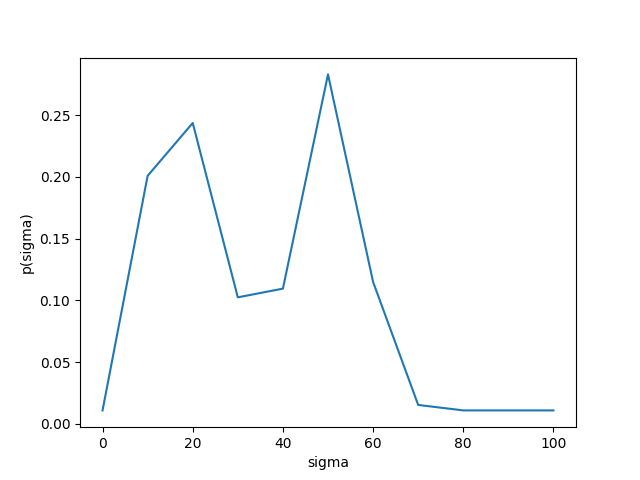
\includegraphics[width=0.5\textwidth]{figs/threeDipSigma.png}
	\caption{A similar proposed curve to \ref{onePeakSigma}.}
	\label{}
\end{figure}

\end{document}
%texcount third.tex -inc -sum -1 